% Options for packages loaded elsewhere
\PassOptionsToPackage{unicode}{hyperref}
\PassOptionsToPackage{hyphens}{url}
\PassOptionsToPackage{dvipsnames,svgnames*,x11names*}{xcolor}
%
\documentclass[
  11pt,
]{article}
\usepackage[]{mathpazo}
\usepackage{amssymb,amsmath}
\usepackage{ifxetex,ifluatex}
\ifnum 0\ifxetex 1\fi\ifluatex 1\fi=0 % if pdftex
  \usepackage[T1]{fontenc}
  \usepackage[utf8]{inputenc}
  \usepackage{textcomp} % provide euro and other symbols
\else % if luatex or xetex
  \usepackage{unicode-math}
  \defaultfontfeatures{Scale=MatchLowercase}
  \defaultfontfeatures[\rmfamily]{Ligatures=TeX,Scale=1}
\fi
% Use upquote if available, for straight quotes in verbatim environments
\IfFileExists{upquote.sty}{\usepackage{upquote}}{}
\IfFileExists{microtype.sty}{% use microtype if available
  \usepackage[]{microtype}
  \UseMicrotypeSet[protrusion]{basicmath} % disable protrusion for tt fonts
}{}
\makeatletter
\@ifundefined{KOMAClassName}{% if non-KOMA class
  \IfFileExists{parskip.sty}{%
    \usepackage{parskip}
  }{% else
    \setlength{\parindent}{0pt}
    \setlength{\parskip}{6pt plus 2pt minus 1pt}}
}{% if KOMA class
  \KOMAoptions{parskip=half}}
\makeatother
\usepackage{xcolor}
\IfFileExists{xurl.sty}{\usepackage{xurl}}{} % add URL line breaks if available
\IfFileExists{bookmark.sty}{\usepackage{bookmark}}{\usepackage{hyperref}}
\hypersetup{
  pdftitle={Data Science Project Guide: Airbnb},
  pdfauthor={TechAcademy e.V.},
  colorlinks=true,
  linkcolor=Maroon,
  filecolor=Maroon,
  citecolor=Blue,
  urlcolor=blue,
  pdfcreator={LaTeX via pandoc}}
\urlstyle{same} % disable monospaced font for URLs
\usepackage[top=0.5in, bottom=1.5in, left=1in, right=1in, a4paper]{geometry}
\usepackage{longtable,booktabs}
% Correct order of tables after \paragraph or \subparagraph
\usepackage{etoolbox}
\makeatletter
\patchcmd\longtable{\par}{\if@noskipsec\mbox{}\fi\par}{}{}
\makeatother
% Allow footnotes in longtable head/foot
\IfFileExists{footnotehyper.sty}{\usepackage{footnotehyper}}{\usepackage{footnote}}
\makesavenoteenv{longtable}
\usepackage{graphicx,grffile}
\makeatletter
\def\maxwidth{\ifdim\Gin@nat@width>\linewidth\linewidth\else\Gin@nat@width\fi}
\def\maxheight{\ifdim\Gin@nat@height>\textheight\textheight\else\Gin@nat@height\fi}
\makeatother
% Scale images if necessary, so that they will not overflow the page
% margins by default, and it is still possible to overwrite the defaults
% using explicit options in \includegraphics[width, height, ...]{}
\setkeys{Gin}{width=\maxwidth,height=\maxheight,keepaspectratio}
% Set default figure placement to htbp
\makeatletter
\def\fps@figure{htbp}
\makeatother
\setlength{\emergencystretch}{3em} % prevent overfull lines
\providecommand{\tightlist}{%
  \setlength{\itemsep}{0pt}\setlength{\parskip}{0pt}}
\setcounter{secnumdepth}{5}
\newcommand{\sectionbreak}{\clearpage}
\usepackage{booktabs}
\RequirePackage{fix-cm}
\usepackage[many]{tcolorbox}
\usepackage{xcolor}

\definecolor{r}{HTML}{2369bd}
\definecolor{p}{HTML}{ffde4d}
\definecolor{boxgrey}{HTML}{fefefe}

\newtcolorbox{rbox}{
  colback=boxgrey,
  colframe=r,
  coltext=black,
  boxsep=5pt,
  arc=4pt}
  
\newtcolorbox{pbox}{
  colback=boxgrey,
  colframe=p,
  coltext=black,
  boxsep=5pt,
  arc=4pt}


\newenvironment{tips}[1]
  {
  \begin{itemize}
  \footnotesize
  \renewcommand{\labelitemi}{
    \raisebox{-.7\height}[0pt][0pt]{
      {\setkeys{Gin}{width=3em,keepaspectratio}
        \includegraphics{images/#1.png}}
    }
  }
  \setlength{\fboxsep}{1em}
  \begin{rbox}
  \item
  }
  {
  \end{rbox}
  \end{itemize}
  }
  
  
\newenvironment{tipsp}[1]
  {
  \begin{itemize}
  \footnotesize
  \renewcommand{\labelitemi}{
    \raisebox{-.7\height}[0pt][0pt]{
      {\setkeys{Gin}{width=3em,keepaspectratio}
        \includegraphics{images/#1.png}}
    }
  }
  \setlength{\fboxsep}{1em}
  \begin{pbox}
  \item
  }
  {
  \end{pbox}
  \end{itemize}
  }
  
\usepackage{fancyhdr}
\pagestyle{fancyplain}
\usepackage{setspace}
\usepackage{chngcntr}
\onehalfspacing

\usepackage{titling}
\pretitle{\begin{center}\LARGE
\includegraphics[width=6cm]{plot/TA_Logo.png}\\[\bigskipamount]}
\posttitle{\end{center}}
\usepackage[]{natbib}
\bibliographystyle{apalike}

\title{Data Science Project Guide: Airbnb}
\author{TechAcademy e.V.}
\date{Winter Term 2021/22}

\begin{document}
\maketitle

\clearpage

\addtolength{\headheight}{17.82275pt}
\rhead{\includegraphics[height=0.5cm]{plot/TA_logo.png}}

\fancyfoot{}
\fancyfoot[R]{\thepage}
\addtolength{\headheight}{17.82275pt}

\fancyfoot[L]{Data Science Project Guide | Airbnb | \copyright\ 2021, TechAcademy e.V.}

\renewcommand{\headrulewidth}{0.25pt}
\renewcommand{\footrulewidth}{0.25pt}

\tableofcontents
\clearpage

\hypertarget{welcome}{%
\section{Welcome!}\label{welcome}}

In the first few chapters, we will introduce you to the basics of the \texttt{R} and \texttt{Python} tracks, and you will find helpful explanations to questions you might have at the beginning of your coding journey.
There will be a quick introduction to the Data Science track so that you can get started with the project quickly.
So let's start with the basics!

In all tracks, you will work on your project in small groups of fellow students.
Such group work helps you finish the project faster and makes your results better.
Our experience shows: The members' different backgrounds and discussing different opinions and ideas will produce the best results.
Besides, it is more fun to work on a project together than to code alone.

The groups can consist of a maximum of three members.
You can choose your two teammates yourself, and we won't interfere with your arrangements.
All group members must complete the same difficulty level (beginner or advanced track) since the tasks are different for each track.
We encourage you to collaborate with students from various departments.
This interdisciplinarity allows you to get to know people from other departments, giving you a whole new perspective on the project and tasks.\\

It is essential to note that each person must submit the project individually for a certificate when submitting your project.
However, each person's project can look identical to the other members of your group.
You will get more information at our first Coding Meetup on \textbf{November 24, 2021}.

This Airbnb case study and its project guide were developed and written from scratch by TechAcademy's Data Science team.
\href{linkedin.com/in/lara-zaremba}{Lara Zaremba}, \href{linkedin.com/in/lukas-juergensmeier}{Lukas Jürgensmeier}, \href{linkedin.com/in/annalisastrauss}{Annalisa Strauß}, \href{linkedin.com/in/karlo-lukic}{Karlo Lukic}, and \href{linkedin.com/in/inga-l-544713180}{Inga Lasys} developed the project in \texttt{R}, while \href{linkedin.com/in/flxschneider}{Felix Schneider}, \href{linkedin.com/in/manuel-mair-am-tinkhof-7b764111b}{Manuel Mair am Tinkhof}, and \href{linkedin.com/in/thilo-leitzbach}{Thilo Leitzbach} developed it in \texttt{Python}.
We would also like to thank \href{linkedin.com/in/benjamin-lucht}{Benjamin Lucht} for his extensive input in making this project a reality.

\hypertarget{whats-data-science-and-how-do-i-do-it}{%
\section{What's Data Science and How Do I Do It?}\label{whats-data-science-and-how-do-i-do-it}}

Data Science is a multi-layered field in which the latest machine learning methods are only a tiny part.
To finish your data science analysis, you'll need to complete many steps -- from collecting to manipulating to exploring the data.
And eventually, you will need to communicate your findings somehow.

But first things first.
To analyze the data, you must first obtain it.
You need to know where to get it and how to integrate it into your respective tools.
The data is rarely available as it would be necessary for further processing.
Familiarizing yourself with the information available, cleaning it up, and processing it into the desired formats that humans and machines can read are essential steps that often make up a large part of the data scientist's work.

Before you can analyze the obtained data, you must first select and master the right tool: the programming language.
The most often used languages for Data Science are \texttt{R}, which was explicitly developed for statistics, and \texttt{Python}, which is characterized by its additional versatility.
The data scientist does not have to be a perfect software developer who masters every detail and programing paradigm.
Still, the competent handling of syntax (writing code) and idiosyncrasies is essential for her.

There are some well-developed method collections, the so-called packages or libraries, which provide a lot of additional functionality to an elemental programing language.
As a data scientist, you should also learn and master the use of these collections, especially when preparing the data.
Once you have prepared your data, you can finally analyze it.

It is also crucial to know and understand the multitude of statistical approaches to choose the correct method for the problem at hand.
The newest, best, and most beautiful neural network is not always the solution to everything!
One step is still missing in the data science process: understanding and communicating your results.
The results are often not spontaneously intuitive or sometimes even surprising.
Here, the data scientist employs specific expertise and creativity, especially during data visualization.

\hypertarget{whats-r}{%
\subsection{What's R?}\label{whats-r}}

\texttt{R} is a programming language developed by statisticians in the early 90s to calculate and visualize statistical results.
A lot has happened since then, and by now, \texttt{R} is one of the most widely used programming languages in Data Science.
You don't have to compile your `R' code, but you can use it interactively and dynamically.
Such an approach makes it possible to quickly gain basic knowledge about existing data and display it graphically.

\texttt{R} offers much more than just programming.
The language provides a complete ecosystem for solving statistical problems.
A large number of packages and interfaces are available, which you can use to expand the basic functionality of the programing language to, say, create a COVID-Tracker application.

\hypertarget{rstudio-cloud}{%
\subsubsection{RStudio Cloud}\label{rstudio-cloud}}

Before you can use \texttt{R}, you usually have to install some separate programs locally on your computer.
Typically, you first install a \href{https://rstudio-education.github.io/hopr/starting.html}{``raw'' version} of \texttt{R}.
In theory, you can then start programming.
However, it is challenging to carry out an entire project with a ``raw'' version of R.
That's why there is \href{https://www.rstudio.com/products/rstudio/download/}{RStudio}, a free Integrated Development Environment (IDE) for \texttt{R}.

Such IDE includes many essential features that simplify programming with \texttt{R}.
Among other things, an auto-completion of your code, a friendly user interface, and many expansion options.
Think of R as your car's engine.
And think of RStudio as your car's dashboard that shows fancy metrics, has a radio and allows you to adjust air-conditioning!

Experience has shown that installing \texttt{R} and RStudio locally on your computer takes some effort.
Fortunately, RStudio also has a cloud solution that eliminates these steps: \href{https://rstudio.cloud}{RStudio Cloud}.
You can edit your project in the same IDE in the browser without any prior installations on your computer.
You can also easily switch your project from a private to a public project and give your team an insight into your code via a link or by giving them access to the workspace directly.
In this way, you can easily exchange ideas with your team.

We will introduce RStudio Cloud and unlock access to our workspace on our first Coding Meetup.
Until then, focus on learning the ``hard skills'' of programming with the courses on DataCamp.
That brings us to your curriculum in the next section!

\hypertarget{curriculum}{%
\subsubsection{Curriculum}\label{curriculum}}

The following list shows the required DataCamp courses for the Data Science with \texttt{R} Track at TechAcademy.
As a beginner, please stick to the courses of the ``beginner'' program.
Ambitious beginners can, of course, take the advanced courses afterward.
However, it would be best if you worked through the courses in the order we listed them.

The same applies to the advanced courses.
Here, too, you should finish the specified courses in the given order.
Since it can, of course, happen that you have already mastered the topics of an advanced course, you can replace some courses.
If you are convinced that the course does not add value to you, feel free to replace it with one of the courses in the ``Exchange Pool'' (see list below).
However, you should not pursue an exchange course until you finish all chapters from the advanced course: ``Intermediate R.''

To receive the certificate, both beginners and advanced learners must complete at least two-thirds of the curriculum (6/9 courses).
For the beginners, this means until -- and including -- the course ``Data Visualization with ggplot2 (Part 1)'' and for the advanced until --and including -- ``Supervised Learning in \texttt{R}: Classification.'' In addition, you should complete at least two-thirds of the project tasks.
After completing the curriculum and the project's (minimal) requirements, you will receive your TechAcademy certificate!

\begin{tips}r

\textbf{R Fundamentals (Beginner Track)}

\begin{enumerate}
\def\labelenumi{\arabic{enumi}.}
\tightlist
\item
  \href{https://www.datacamp.com/courses/free-introduction-to-r}{Introduction to R (4h)}
\item
  \href{https://www.datacamp.com/courses/intermediate-r}{Intermediate R (6h)}
\item
  \href{https://www.datacamp.com/courses/importing-data-in-r-part-1}{Introduction to Importing Data in R (3h)}
\item
  \href{https://www.datacamp.com/courses/cleaning-data-in-r}{Cleaning Data in R (4h)}
\item
  \href{https://www.datacamp.com/courses/data-manipulation-with-dplyr-in-r}{Data Manipulation with dplyr (4h)}
\item
  \href{https://www.datacamp.com/courses/data-visualization-with-ggplot2-1}{Data Visualization with ggplot2 (Part1) (5h)}
\item
  \href{https://www.datacamp.com/courses/exploratory-data-analysis}{Exploratory Data Analysis in R (4h)}
\item
  \href{https://www.datacamp.com/courses/correlation-and-regression}{Correlation and Regression in R (4h)}
\item
  \href{https://www.datacamp.com/courses/multiple-and-logistic-regression}{Multiple and Logistic Regression in R (4h)}
\end{enumerate}

\textbf{Machine Learning Fundamentals in R (Advanced Track)}

\begin{enumerate}
\def\labelenumi{\arabic{enumi}.}
\tightlist
\item
  \href{https://www.datacamp.com/courses/intermediate-r}{Intermediate R (6h)}
\item
  \href{https://www.datacamp.com/courses/importing-data-in-r-part-1}{Introduction to Importing Data in R (3h)}
\item
  \href{https://www.datacamp.com/courses/cleaning-data-in-r}{Cleaning Data in R (4h)}
\item
  \href{https://www.datacamp.com/courses/importing-cleaning-data-in-r-case-studies}{Importing \& Cleaning Data in R: Case Studies (4h)}
\item
  \href{https://www.datacamp.com/courses/data-visualization-with-ggplot2-1}{Data Visualization with ggplot2 (Part1) (5h)}
\item
  \href{https://www.datacamp.com/courses/supervised-learning-in-r-classification}{Supervised Learning in R: Classification (4h)}
\item
  \href{https://www.datacamp.com/courses/supervised-learning-in-r-regression}{Supervised learning in R: Regression (4h)}
\item
  \href{https://www.datacamp.com/courses/unsupervised-learning-in-r}{Unsupervised Learning in R (4h)}
\item
  \href{https://www.datacamp.com/courses/machine-learning-toolbox}{Machine Learning with caret in R (4h)}
\end{enumerate}

\textbf{Data Science R (Advanced Track) -- Exchange Pool}

\begin{itemize}
\tightlist
\item
  \href{https://www.datacamp.com/courses/data-visualization-with-ggplot2-2}{Data Visualization with ggplot2 (Part 2) (5h)}
\item
  \href{https://www.datacamp.com/courses/interactive-maps-with-leaflet-in-r}{Interactive Maps with leaflet in R (4h)}
\item
  \href{https://www.datacamp.com/courses/machine-learning-in-the-tidyverse}{Machine Learning in Tidyverse (5h)}
\item
  \href{https://www.datacamp.com/courses/writing-efficient-r-code}{Writing Efficient R Code (4h)}
\item
  \href{https://www.datacamp.com/courses/support-vector-machines-in-r}{Support Vector Machines in R (4h)}
\item
  \href{https://www.datacamp.com/courses/supervised-learning-in-r-case-studies}{Supervised Learning in R: Case Studies (4h)}
\item
  \href{https://www.datacamp.com/courses/optimizing-r-code-with-rcpp}{Optimizing R Code with Rcpp (4h)}
\end{itemize}


\end{tips}

\hypertarget{helpful-links}{%
\subsubsection{Helpful Links}\label{helpful-links}}

\begin{itemize}
\tightlist
\item
  \href{https://rstudio.cloud/learn/cheat-sheets}{RStudio Cheat Sheets}
\item
  \href{https://rmarkdown.rstudio.com/lesson-1.html}{RMarkdown Explanation} (to document your analyses)
\item
  \href{https://stackoverflow.com/}{StackOverflow} (forum for all kinds of coding questions)
\item
  \href{https://stats.stackexchange.com/}{CrossValidated} (Statistics and Data Science forum)
\end{itemize}

\hypertarget{whats-python}{%
\subsection{What's Python?}\label{whats-python}}

\texttt{Python} is a dynamic programming language.
You can execute the code in the interpreter, so you do not have to compile the code first.
This feature makes \texttt{Python} very easy and quick to use.
The excellent usability, easy readability, and simple structuring were and still are core ideas in developing this programming language.

You can use \texttt{Python} to program according to any paradigm, whereby structured and object-oriented programming is most straightforward due to the structure of the language.
Still, functional or aspect-oriented programming is also possible.
These options give users significant freedom to design projects the way they want and great space to write code that is difficult to understand and confusing.
For this reason, programmers developed specific standards based on the so-called \texttt{Python} Enhancement Proposals (PEP) over the decades.

\hypertarget{anaconda-and-jupyter}{%
\subsubsection{Anaconda and Jupyter}\label{anaconda-and-jupyter}}

Before you can use \texttt{Python}, you must install it on the computer.
\texttt{Python} is already installed on Linux and Unix systems (such as macOS), but often it is an older version.
Since there are differences in the handling of \texttt{Python} version 2 -- which is no longer supported -- and version 3, we decided to work with version 3.6 or higher.

One of the easiest ways to get Python and most of the best-known programming libraries is to install Anaconda.
There are detailed explanations for installing all operating systems on the \href{https://docs.anaconda.com/anaconda/install/}{website} of the provider.

With Anaconda installed, all you have to do is open the Anaconda Navigator, and you're ready to go.
There are two ways to get started: Spyder or Jupyter.
Spyder is the integrated development environment (IDE) for \texttt{Python} and offers all possibilities from syntax highlighting to debugging (links to tutorials below).

The other option is to use Jupyter or Jupyter notebooks.
It is an internet technology-based interface for executing commands.
The significant advantage of this is that you can quickly write shortcode pieces and try them out interactively without writing an entire executable program.
Now you can get started!

If you have not worked with Jupyter before, we recommend that you complete \href{https://app.datacamp.com/learn/projects/introduction-to-projects/guided/Python}{this DataCamp course} first.
There you will get to know many tips and tricks that will make your workflow with Jupyter much easier.

To make your work and, above all, the collaboration more accessible, we are working with the \href{https://colab.research.google.com/notebooks/basic_features_overview.ipynb}{Google Colab} platform that contains a Jupyter environment with the necessary libraries.
You can then import all the data required for the project with Google Drive.
We will introduce this environment during our first Coding Meetup.
Until then, focus on learning the ``hard skills'' of programming with your courses on DataCamp.
This topic brings us to your curriculum in the next section!

\hypertarget{curriculum-1}{%
\subsubsection{Curriculum}\label{curriculum-1}}

The following list shows the required DataCamp courses for the Data Science with \texttt{Python} Track at TechAcademy.
As a beginner, please stick to the courses of the ``beginner'' program.
Ambitious beginners can, of course, take the advanced courses afterward.
However, it would be best if you worked through the courses in the order we listed them.

The same applies to the advanced courses.
Here, too, you should finish the specified courses in the given order.
Since it can, of course, happen that you have already mastered the topics of an advanced course, you can replace some courses.
If you are convinced that the course does not add value to you, feel free to replace it with one of the courses in the ``Exchange Pool'' (see list below).
However, you should not pursue an exchange course until you finish all chapters from the advanced course: ``Intermediate Python.''

To receive the certificate, both beginners and advanced learners must complete at least two-thirds of the curriculum (6/9 courses).
For the beginners, this means until -- and including -- the course ``\href{https://learn.datacamp.com/courses/merging-dataframes-with-pandas}{Merging DataFrames with pandas (4h)}'' and for the advanced until --and including -- ``\href{https://learn.datacamp.com/courses/exploratory-data-analysis-in-python}{Exploratory Data Analysis in Phyton (4h)}.'' In addition, you should complete at least two-thirds of the project tasks.
After completing the curriculum and the project's (minimal) requirements, you will receive your TechAcademy certificate!

\begin{tipsp}p

\textbf{Python Fundamentals (Beginner Track)}

\begin{enumerate}
\def\labelenumi{\arabic{enumi}.}
\tightlist
\item
  \href{https://www.datacamp.com/courses/introduction-to-data-science-in-python}{Introduction to Data Science in Python (4h)}
\item
  \href{https://www.datacamp.com/courses/intermediate-python-for-data-science}{Intermediate Python (4h)}
\item
  \href{https://www.datacamp.com/courses/python-data-science-toolbox-part-1}{Python for Data Science Toolbox (Part 1) (3h)}
\item
  \href{https://www.datacamp.com/courses/introduction-to-matplotlib}{Introduction to Data Visualization with Matplotlib (4h)}
\item
  \href{https://www.datacamp.com/courses/manipulating-dataframes-with-pandas}{Manipulating DataFrames with pandas (4h)}
\item
  \href{https://www.datacamp.com/courses/merging-dataframes-with-pandas}{Merging DataFrames with pandas (4h)}
\item
  \href{https://www.datacamp.com/courses/exploratory-data-analysis-in-python}{Exploratory Data Analysis in Phyton (4h)}
\item
  \href{https://www.datacamp.com/projects/33}{Introduction to DataCamp Projects (2h)}
\item
  \href{https://www.datacamp.com/courses/introduction-to-linear-modeling-in-python}{Introduction to Linear Modeling in Python (4h)}
\end{enumerate}

\textbf{Data Science with Python (Advanced Track)}

\begin{enumerate}
\def\labelenumi{\arabic{enumi}.}
\tightlist
\item
  \href{https://www.datacamp.com/courses/intermediate-python-for-data-science}{Intermediate Python (4h)}
\item
  \href{https://www.datacamp.com/courses/python-data-science-toolbox-part-1}{Python Data Science Toolbox (Part 1) (3h)}
\item
  \href{https://www.datacamp.com/courses/python-data-science-toolbox-part-2}{Python Data Science Toolbox (Part 2) (4h)}
\item
  \href{https://www.datacamp.com/courses/cleaning-data-in-python}{Cleaning Data in Python (4h)}
\item
  \href{https://www.datacamp.com/projects/82}{Exploring the Bitcoin Cryptocurrency Market (3h)}
\item
  \href{https://www.datacamp.com/courses/exploratory-data-analysis-in-python}{Exploratory Data Analysis in Phyton (4h)}
\item
  \href{https://www.datacamp.com/courses/introduction-to-linear-modeling-in-python}{Introduction to Linear Modeling in Python (4h)}
\item
  \href{https://www.datacamp.com/courses/supervised-learning-with-scikit-learn}{Supervised Learning with Scikit-Learn (4h)}
\item
  \href{https://www.datacamp.com/courses/linear-classifiers-in-python}{Linear Classifiers in Python (4h)}
\end{enumerate}

\textbf{Data Science with Python (Advanced Track) - Exchange Pool}

\begin{itemize}
\tightlist
\item
  \href{https://www.datacamp.com/projects/684}{TV, Halftime Shows and the Big Game (4h)}
\item
  \href{https://www.datacamp.com/courses/interactive-data-visualization-with-bokeh}{Interactive Data Visualization with Bokeh (4h)}
\item
  \href{https://www.datacamp.com/courses/introduction-to-time-series-analysis-in-python}{Time Series Analysis (4h)}
\item
  \href{https://www.datacamp.com/courses/machine-learning-for-time-series-data-in-python}{Machine Learning for Time Series Data in Python (4h)}
\item
  \href{https://www.datacamp.com/courses/advanced-deep-learning-with-keras-in-python}{Advanced Deep Learning with Keras (4h)}
\item
  \href{https://www.datacamp.com/courses/data-visualization-with-seaborn}{Data Visualization with Seaborn (4h)}
\item
  \href{https://www.datacamp.com/courses/web-scraping-with-python}{Web Scraping in Python (4h)}
\item
  \href{https://www.datacamp.com/courses/writing-efficient-python-code}{Writing Efficient Python Code (4h)}
\item
  \href{https://www.datacamp.com/courses/unsupervised-learning-in-python}{Unsupervised Learning in Python (4h)}
\item
  \href{https://www.datacamp.com/courses/optimizing-python-code-with-pandas}{Writing Efficient Code with pandas (4h)}
\item
  \href{https://www.datacamp.com/courses/deep-learning-in-python}{Introduction to Deep Learning in Python (4h)}
\item
  \href{https://www.datacamp.com/courses/forecasting-using-arima-models-in-python}{ARIMA Models in Python (4h)}
\end{itemize}


\end{tipsp}

\hypertarget{helpful-links-1}{%
\subsubsection{Helpful Links}\label{helpful-links-1}}

Official Tutorials/Documentation:

\begin{itemize}
\tightlist
\item
  \url{https://docs.python.org/3/tutorial/index.html}
\item
  \url{https://jupyter.org/documentation}
\end{itemize}

Further Explanations:

\begin{itemize}
\tightlist
\item
  \url{https://pythonprogramming.net/}
\item
  \url{https://automatetheboringstuff.com/}
\item
  \url{https://www.reddit.com/r/learnpython}
\item
  \url{https://www.datacamp.com/community/tutorials/tutorial-jupyter-notebook}
\end{itemize}

\hypertarget{your-data-science-project}{%
\subsection{Your Data Science Project}\label{your-data-science-project}}

\hypertarget{coding-meetups-and-requirements}{%
\subsubsection{Coding Meetups and Requirements}\label{coding-meetups-and-requirements}}

Now that you have learned the theoretical foundation of Data Science in the DataCamp courses, you can put your skills into practice.
We have put together a project for you based on real data sets.
You can read about the details of this project in the following chapters of this project guide.

Of course, we will also describe the project and the tools that go with it.
We will discuss everything you need to know during the first Coding Meetup, which will take place on \textbf{November 24, 2021}.
After that, your work on the project will officially begin.
You can find the exact project tasks together with further explanations and hints in the following chapters.

To receive your TechAcademy certificate, you must solve at least two-thirds of the ``Exploratory Data Analysis'' part of your Data Science project.
We added the ``Price Prediction -- The Application of Statistical Models'' part for the advanced participants.
In addition, you should complete two-thirds (6/9 courses) of the respective curriculum on DataCamp, as mentioned.
You can find more detailed information about the curriculum in the ``Curriculum'' section of the different programming languages above.

\newpage

\hypertarget{introduction-to-your-project}{%
\section{Introduction to Your Project}\label{introduction-to-your-project}}

\hypertarget{purpose-of-the-project-guide}{%
\subsection{Purpose of the Project Guide}\label{purpose-of-the-project-guide}}

Welcome to the project guide for your TechAcademy Data Science project!
This document will guide you through the different steps of your project and provide you with valuable hints along the way.
However, the guide is not a detailed step-by-step manual.
We think you should develop the skills of coming up with your way of solving different tasks.
Such an approach is an excellent opportunity to apply the knowledge and tools you acquired through DataCamp.

Questions might come up, or you might not know how to solve a task right away - but do not worry - that is just a part of coding.
In those cases, you can find helpful links in the introductory chapters, where someone might have answered your question(s).
If not -- and in the unlikely case that even Google cannot provide the answer -- our TechAcademy mentors will help you via Slack or directly during the coding meetups.
You are strongly encouraged to chat with your group's mentors!

\textbf{At the end of the project guide, you will find an overview of the tasks you must complete}, depending on your track (beginner vs.~advanced).
You can use that list to check which tasks you still need to complete or which assignments are relevant for your track.

\hypertarget{what-is-this-project-about}{%
\subsection{What is this Project About?}\label{what-is-this-project-about}}

Having worked with Spotify data last semester, we will focus on a different topic this semester: \textbf{Airbnb}.
More precisely, you will analyze data about Airbnb offers in a city of your choice!
You can choose from the following list of cities according to your preferences, but each group member should work on a different city:

Amsterdam, Boston, Edinburgh, Madrid, München, and Rom.

Find the links to all datasets \href{https://docs.google.com/document/d/1nBkeJmpnoiATVw4B3DwrB45uo0TpQFE_iTisyh4p9Ro/edit?usp=sharing}{here}.

Your data was scraped and is hosted by the Inside Airbnb project.
You will find all kinds of information in that data set -- both valuable and worthless to your analysis.
In the analogy of the typical data science workflow, we have split this project into two parts.
First, you are going to learn how to perform an Exploratory Data Analysis (EDA).
You will have a closer look at the data, transform it and then get to know the different variables and how they look in various visualizations.

Beginners will complete the project after this first part.
Still, it would be beneficial for beginners to try and work on the second part too.
In the next part of the project, advanced programmers will develop a model that predicts Airbnb prices in their city as accurately as possible.
They will start with a linear regression algorithm which they can modify as pleased.
Additionally, they will explore other possibilities of modeling and data prediction.

But first things first: What exactly is EDA, and what can you achieve with it?

\hypertarget{exploratory-data-analysis-getting-to-know-the-data-set}{%
\subsection{Exploratory Data Analysis -- Getting to Know the Data Set}\label{exploratory-data-analysis-getting-to-know-the-data-set}}

As a first step, you will get to know the data set.
This step means you will describe the data and answer questions like: What variables does the data set contains?
And how are they related?
For this purpose, you often use graphical tools like box plots or histograms.

We structured the first part of the project to let you know the data thoroughly by completing the given tasks one after the other.
As a beginner, you can stop after this part because you will have fulfilled the necessary coding requirements for your TechAcademy certificate.
However, if this first part inspires you to step up your ``apartment-search game,'' we encourage you to work on the second part!

Since data science concepts are independent of specific programming languages, we will describe the general approach in this part of the text.
Having understood the bigger picture and starting with the tasks, you will find language-specific tips and tricks in visually separated boxes.

If you participate in our \texttt{R}-Track, you will need to look at the boxes with the blue border.
Likewise, you look at the yellow-bordered boxes if you code in \texttt{Python}.
From time to time, it might be interesting to check out the other language -- though you can code the exact solutions in both, they sometimes have a different approach to an identical problem.
It makes sense that you complete the first few beginner chapters mentioned in \href{https://tech-academy-ev.github.io/whats-data-science-and-how-do-i-do-it.html\#whats-data-science-and-how-do-i-do-it}{Section 2}.
We recommend that you finish the courses at least until -- and including -- \emph{Exploratory Data Analysis in \[your programing language of choice\]}.

\hypertarget{prediction-apply-statistical-methods}{%
\subsection{Prediction -- Apply Statistical Methods}\label{prediction-apply-statistical-methods}}

This part of the project is mainly for the advanced TechAcademy participants.
If you are a beginner and have completed the first part and have some leftover motivation, we would love to see you complete the second part too!
Statistical models are a significant part of data science, and this gives you a chance to get acquainted with such frameworks.

As you studied the data in part one, you should be familiar with its features, and you can start creating predictions about Airbnb prices -- based on the information you learned about the apartments.
After completing the second part, you will send us your predictions, and we will check how accurate your model was.
The most precise model wins the race!

For this part of the project, we recommend the advanced courses mentioned in \href{https://tech-academy-ev.github.io/whats-data-science-and-how-do-i-do-it.html\#whats-data-science-and-how-do-i-do-it}{Section 2}.
Please note that even more DataCamp classes are available, so if you want to extend your skills further, feel free to complete more courses on the topics that interest you.
We recommend that you finish the lessons at least until -- and including --\emph{Unsupervised Learning in Python} for the \texttt{Python} track and \emph{Machine Learning Toolbox} for the \texttt{R} track.

Ready to get your hands dirty?
After getting a first impression of what this project is about, let's get you started!

:::

\newpage

\hypertarget{exploratory-data-analysis}{%
\section{Exploratory Data Analysis}\label{exploratory-data-analysis}}

Before you can dive into the data, set up your programming environment.
This will be the place where the magic happens -- all your coding will take place there.

\begin{tips}r
In your workspace on \href{https://rstudio.cloud/projects}{RStudio Cloud}, we have already uploaded an ``assignment'' for you (Template Airbnb).
When you create a new project within the workspace \emph{Class of '21/22 \textbar{} TechAcademy \textbar{} Data Science with R}, your workspace will open up.

We've already made some arrangements for you: The data sets you will be working with throughout the project are already available in your working directory.
We also created an RMarkdown file (a file that ends with \texttt{.Rmd} extension), with which you will be able to create a detailed report of your project.
You can convert that file into an HTML document when you have finished coding the project in R.
Open the file \texttt{Markdown\_Airbnb.Rmd} and see for yourself!

\end{tips}

\begin{tipsp}p
We recommend using \href{https://colab.research.google.com}{Google Colab} for this project since it requires no particular setup, stores its notebooks to your Google Drive, and makes it easy for you to share them with your team members.

As an alternative to Google Colab, you might want to install Jupyter Notebook locally using the Anaconda distribution.
Either way, when importing Airbnb data, you can use the links to the respective data files provided in the ``Data-Links'' document, which you will find in the TechAcademy drive.

We will give you a more detailed step-by-step demo during the first coding meetup.


\end{tipsp}

\hypertarget{visualizing-apartment-availability}{%
\subsection{Visualizing Apartment Availability}\label{visualizing-apartment-availability}}

Imagine being a tourist on a budget.
First things first, you might want to check for periods when apartments (or, Airbnbs) are available for booking on the market.
Remember the basics of economics?
A lower supply of a product on the market usually comes with higher prices (all else equal).
Vice versa, a higher supply of a product might come with a lower price.
That is precisely what you want if you are on a budget!
Explore the data set looking for periods with high availability and find out later whether that basic economic idea holds in the Airbnb context.

\hypertarget{import-clean-and-transform-the-data}{%
\subsubsection{Import, Clean and Transform the Data}\label{import-clean-and-transform-the-data}}

In this chapter, you will apply the knowledge that you gained throughout the semester to real-world data.
The exercises will cover typical problems that you usually encounter when analyzing data.

First things first, you will need to load the \texttt{calendar.csv} file into your coding environment: How is the data structured, and which variables does it contain?
To get a peek at the data you'll be working with, output the first/last few rows.
Also, compute some basic descriptive statistics (e.g., count, mean, and standard deviation) and determine the column's data types.

\begin{tips}r
First, load the necessary packages/libraries that you intended to use for your analysis.

Then, load the data set from your folder structure into the workspace.
Import the calendar data set into your workspace and name the object accordingly.
Use, for example:

\texttt{calendar\ \textless{}-\ read\_csv("calendar.csv")}

Now get an overview of the data set.
How is it structured, and which variables does it contain?
You can use the following functions, for example:

\texttt{head(calendar)}~\\
\texttt{str(calendar)}~\\
\texttt{summary(calendar)}

\end{tips}

\begin{tipsp}p
Import the pandas library to your notebook with \texttt{import\ pandas\ as\ pd}.
Use the same pandas method used to import CSV data on Datacamp to import CSV data from a web server: Just replace the file path with the URL of the CSV file.

Take a look at the first rows of your data frame and print some descriptive statistics with the pandas methods \texttt{.head()} and \texttt{.describe()}.
Also, find out the data types for each column: Are values in the price column stored as numbers?

\end{tipsp}

Visualization is one of the most helpful methods to get a feeling for the relation of the various variables of the data set.
As already mentioned, this process is called \emph{Exploratory Data Analysis} (EDA).

Before starting with that, we first have to clean the data so that the functions can process the data set correctly.
You will have to do that quite often in the field of Data Science since the data very often comes in an unusable format.
For example, in our case, the values in the price column are not stored as a numeric data type -- this becomes an issue when performing math operations on such columns.

\begin{tips}r
In order for \texttt{R} to process this, we need to remove a character from the observations and convert the variable into a numeric format.
You can use the functions \texttt{str\_remove\_all()} or \texttt{gsub()} together with \texttt{as.numeric()} for this.

To make the next step easier, we still have to convert the logical variable \texttt{available} from a \texttt{character} to a \texttt{boolean} data type.
Use, for example, the \texttt{ifelse()} function for this and replace ``f'' and ``t'' with the associated logical values \texttt{FALSE} and \texttt{TRUE}.

As a last step, transform the \texttt{date} variable into the \texttt{R} format \texttt{Date}.
Remember the \texttt{as.numeric()} function?
\texttt{R} has a similar function to convert variables to a date format.

\end{tips}

\begin{tipsp}p
To remove a character in a column's cells use pandas' \texttt{.replace()} method.
Similarly, convert the data to a different type with \texttt{.astype()} (Hint: You might need to apply the replace method twice on the price column before converting).

Note that the column indicating apartment availability contains two values, namely \texttt{f} and \texttt{t}.
Replace \texttt{f} and \texttt{t} with the associated boolean values \texttt{FALSE} and \texttt{TRUE}.

\end{tipsp}

Our goal now is to show the number of Airbnb apartments available over the next year in a simple line plot.
However, this goal is still not possible since there is an entry for each apartment in the upcoming 365 days.
And another related variable that shows us whether the apartment is available or not on each of those days is present too.
The transformed data set should summarize this information and have only one entry for each day that tells us the aggregated number of available Airbnbs in the city.

\begin{tips}r
The \texttt{R} package \texttt{dplyr} is the first choice for this type of transformation task.
If you haven't heard of it yet, take the respective DataCamp course or the DataCamp course on Exploratory Data Analysis.

Use the \texttt{dplyr} functions \texttt{group\_by()} and \texttt{summarize()} and save the resulting data set in a new data frame, which you can call \texttt{avail\_by\_date}.
You can, of course, name the data frame however you wish.

If you need further help, you can also use the \texttt{dplyr} \href{https://www.rstudio.com/wp-content/uploads/2015/02/data-wrangling-cheatsheet.pdf}{Cheat Sheet} for this task, on which you can visually see such transformations.

\end{tips}

\begin{tipsp}p
To understand this step, remember that you converted the values in the \texttt{available} column to be of type \texttt{bool}.
In Python, the boolean value \texttt{True} is equal to \texttt{1}, while \texttt{False} is equal to \texttt{0}.
Thus, \texttt{True\ +\ True\ +\ False} is equal to \texttt{2} (you can try this out by executing \texttt{print(True\ +\ True\ +\ False)}).
So, to get the number of available apartments, you could simply sum the (boolean) values in the \texttt{available} column!

But before doing so, make sure to group the data frame by date with \texttt{.groupby()} in combination with the aggregation method \texttt{.sum()} as you need to get the number of available apartments for each date.

The pandas \href{https://pandas.pydata.org/Pandas_Cheat_Sheet.pdf}{Cheat Sheet} might be of help here - feel free to make use of it.

\end{tipsp}

\hypertarget{days-lineplot}{%
\subsubsection{365 Days Lineplot}\label{days-lineplot}}

We have finally transformed the data set into a useful format, so now it is time to actually visualize it.
We are going to get started with a simple line plot that shows the number of available apartments over the next 365 days.
This is what your result could look like:

\begin{center}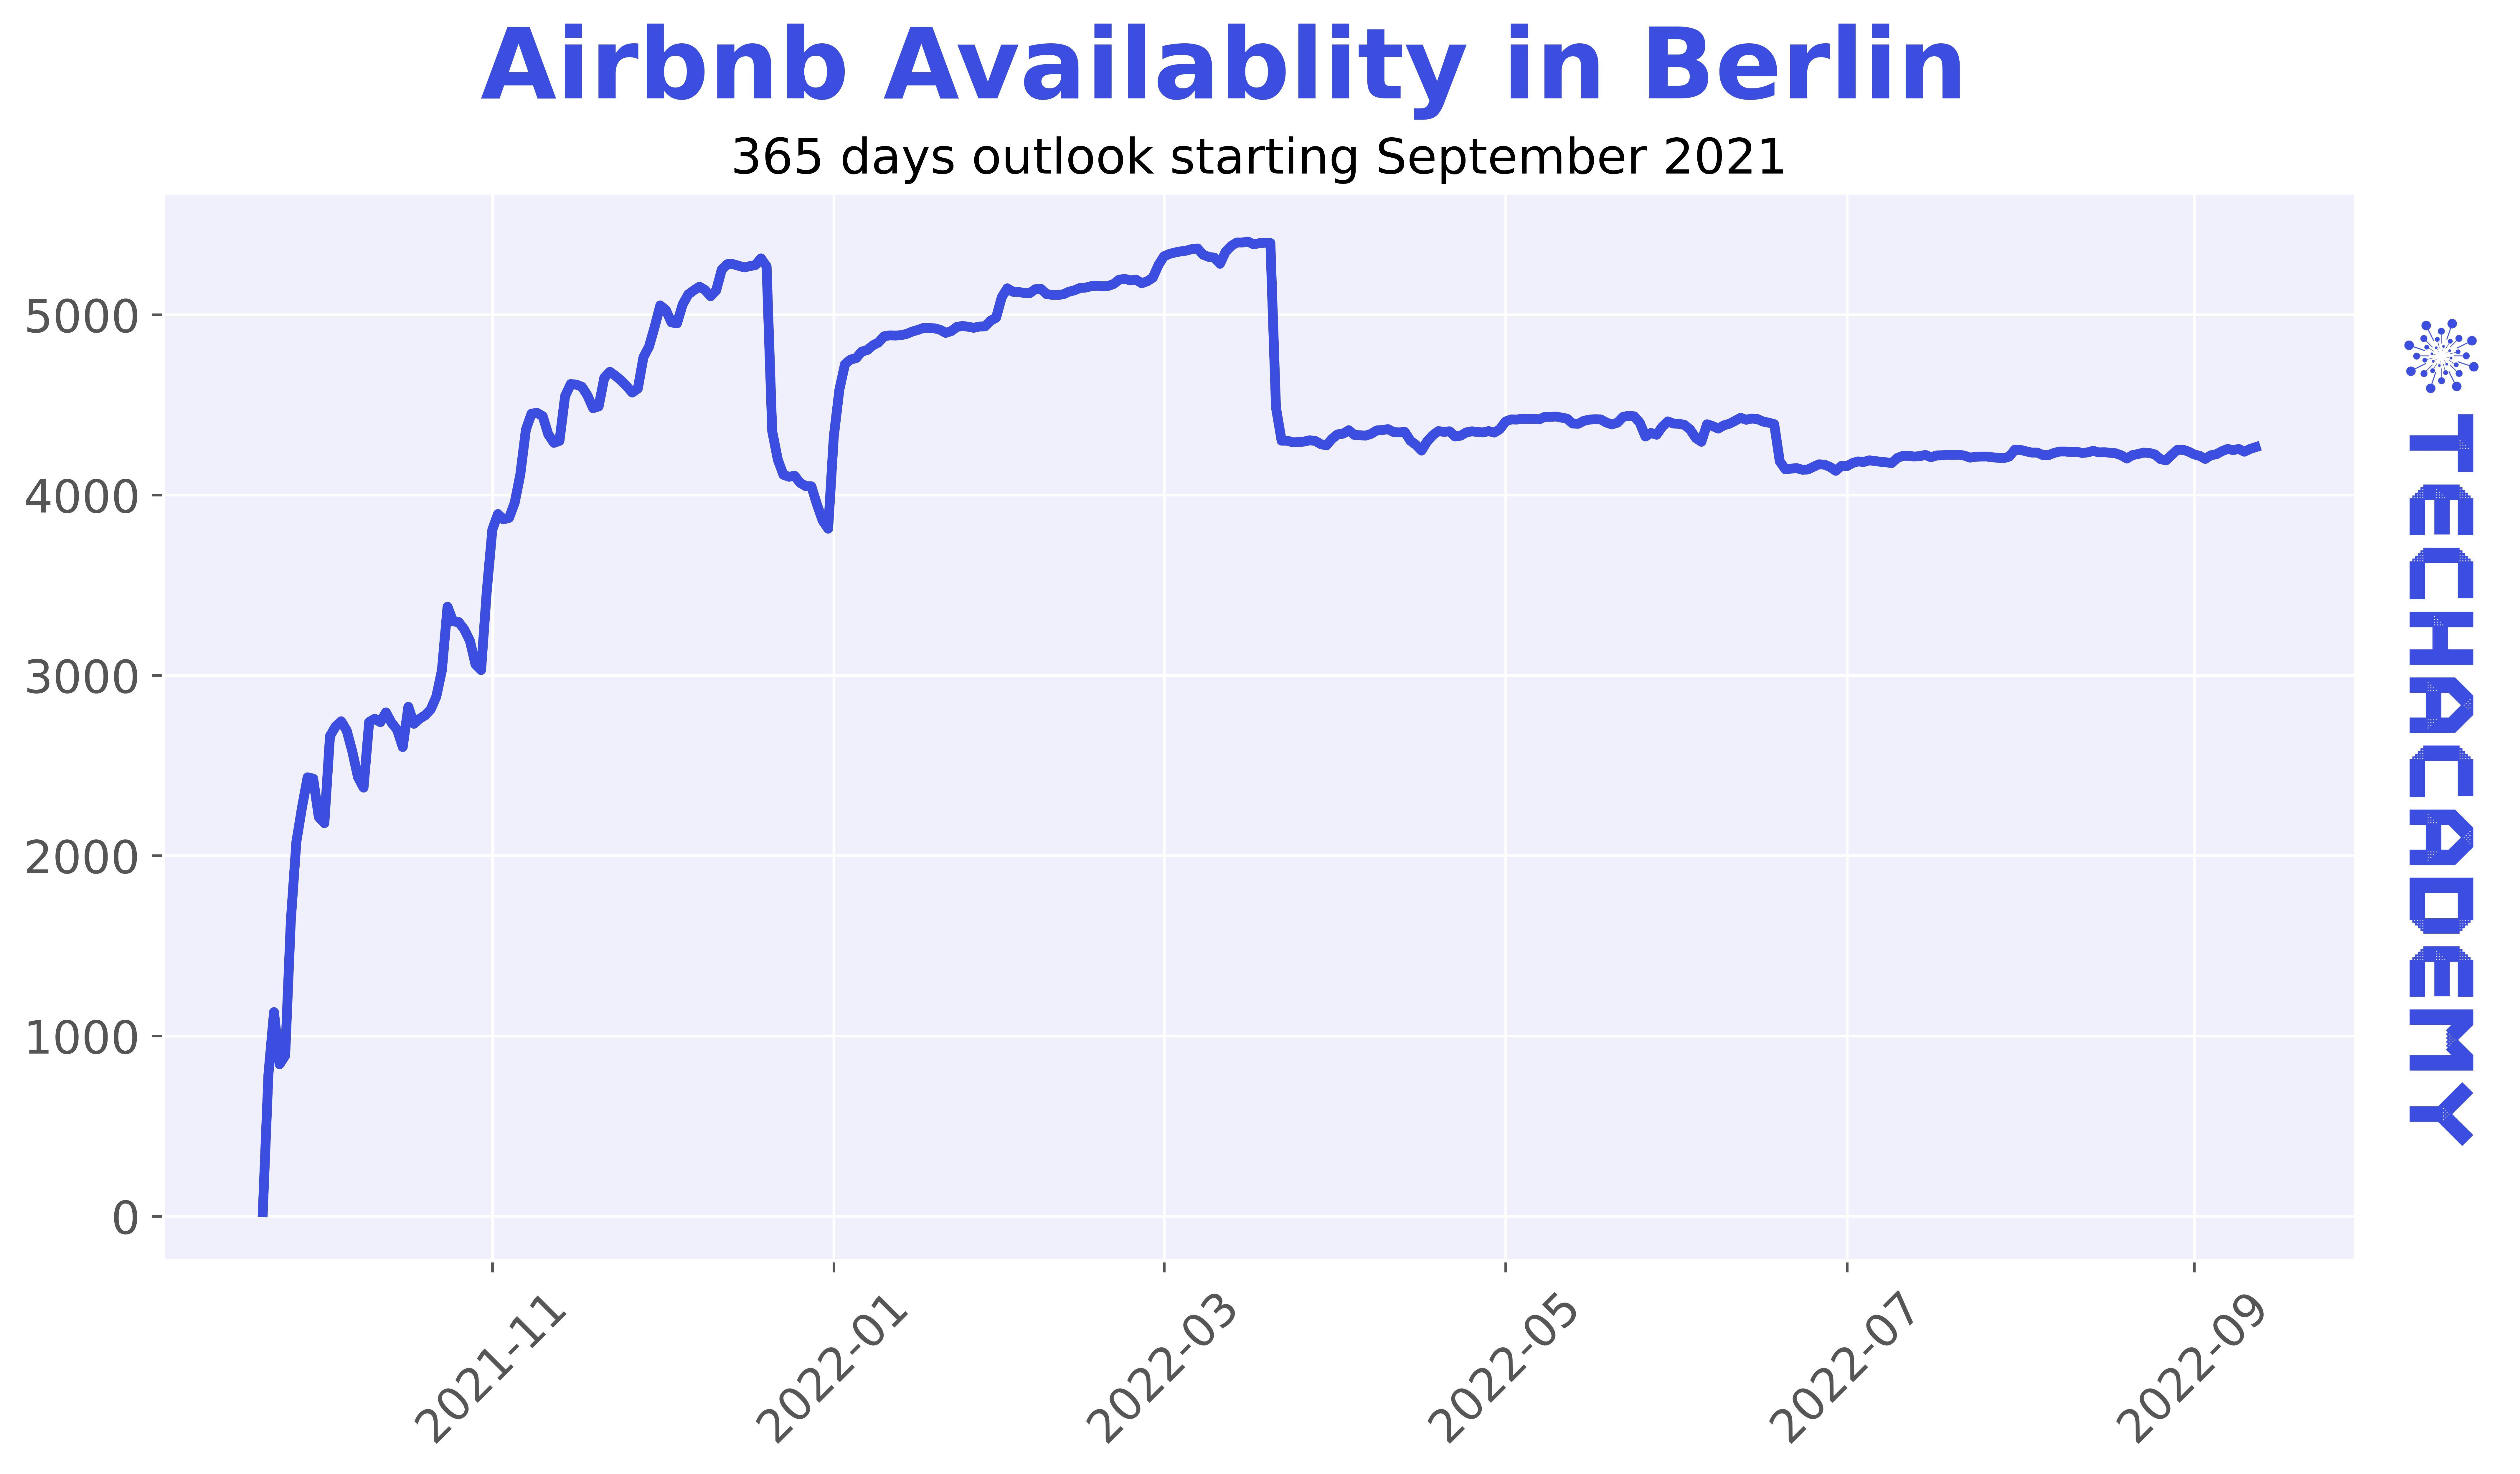
\includegraphics[width=1\linewidth]{plot/01_python/availability} \end{center}

\begin{tips}r
For this visualization, you can use the \texttt{base} package that includes the function \texttt{plot()} or use the more extensive and very flexible graphics package \texttt{ggplot2}.
We highly recommend getting comfortable with using the\texttt{ggplot2} package as it's one of the most used \texttt{R} packages overall.

\end{tips}

\begin{tipsp}p
Having the data in the correct format, we can now start plotting a simple line graph.
For this, you can use matplotlib's \texttt{plt.plot()}.

\end{tipsp}

Looking at the line plot above, you can see a clear pattern for different dates.
There are distinct drops in the availability of Airbnb apartments.~
\textbf{One task for your project is to think about a potential cause behind this pattern: Is there one?}

\hypertarget{calendar-plot}{%
\subsubsection{Calendar Plot}\label{calendar-plot}}

A line plot is good but let's be honest; it's nothing to write home about!
How about using a calendar plot to get a quick overview of this year's most and least abundant Airbnb months?
Let's see:

\begin{center}
\includegraphics[width=1\linewidth]{plot/01_python/calendar} \end{center}

There are country-specific holidays and seasons, after all!

\begin{tips}r
Check out the \href{https://r-coder.com/calendar-plot-r/}{calendR} \texttt{R} package to visualize the availability of Airbnb listings in a calendar plot.

\end{tips}

\begin{tipsp}p
You can use the package \href{https://pythonhosted.org/calmap/}{calmap} to visualize availability in an intuitive manner!

\end{tipsp}

\hypertarget{correlation-coefficient-and-plot}{%
\subsection{Correlation Coefficient and Plot}\label{correlation-coefficient-and-plot}}

Now that you are confident that there are some distinct patterns in the data set, you might be willing to quantify your suspicion.
For that purpose, calculate the correlation coefficient (\emph{r}) between \texttt{availability} and \texttt{price} and plot both variables to confirm your intuition.

Regarding visualization, you could, for example, choose between:

a) line plot (boring as you already did it), or

b) scatter plot (exciting as it's something new for you).

Please \textbf{write a short sentence explaining what the correlation coefficient measures in this context.}

For example, this task could look like:

\begin{center}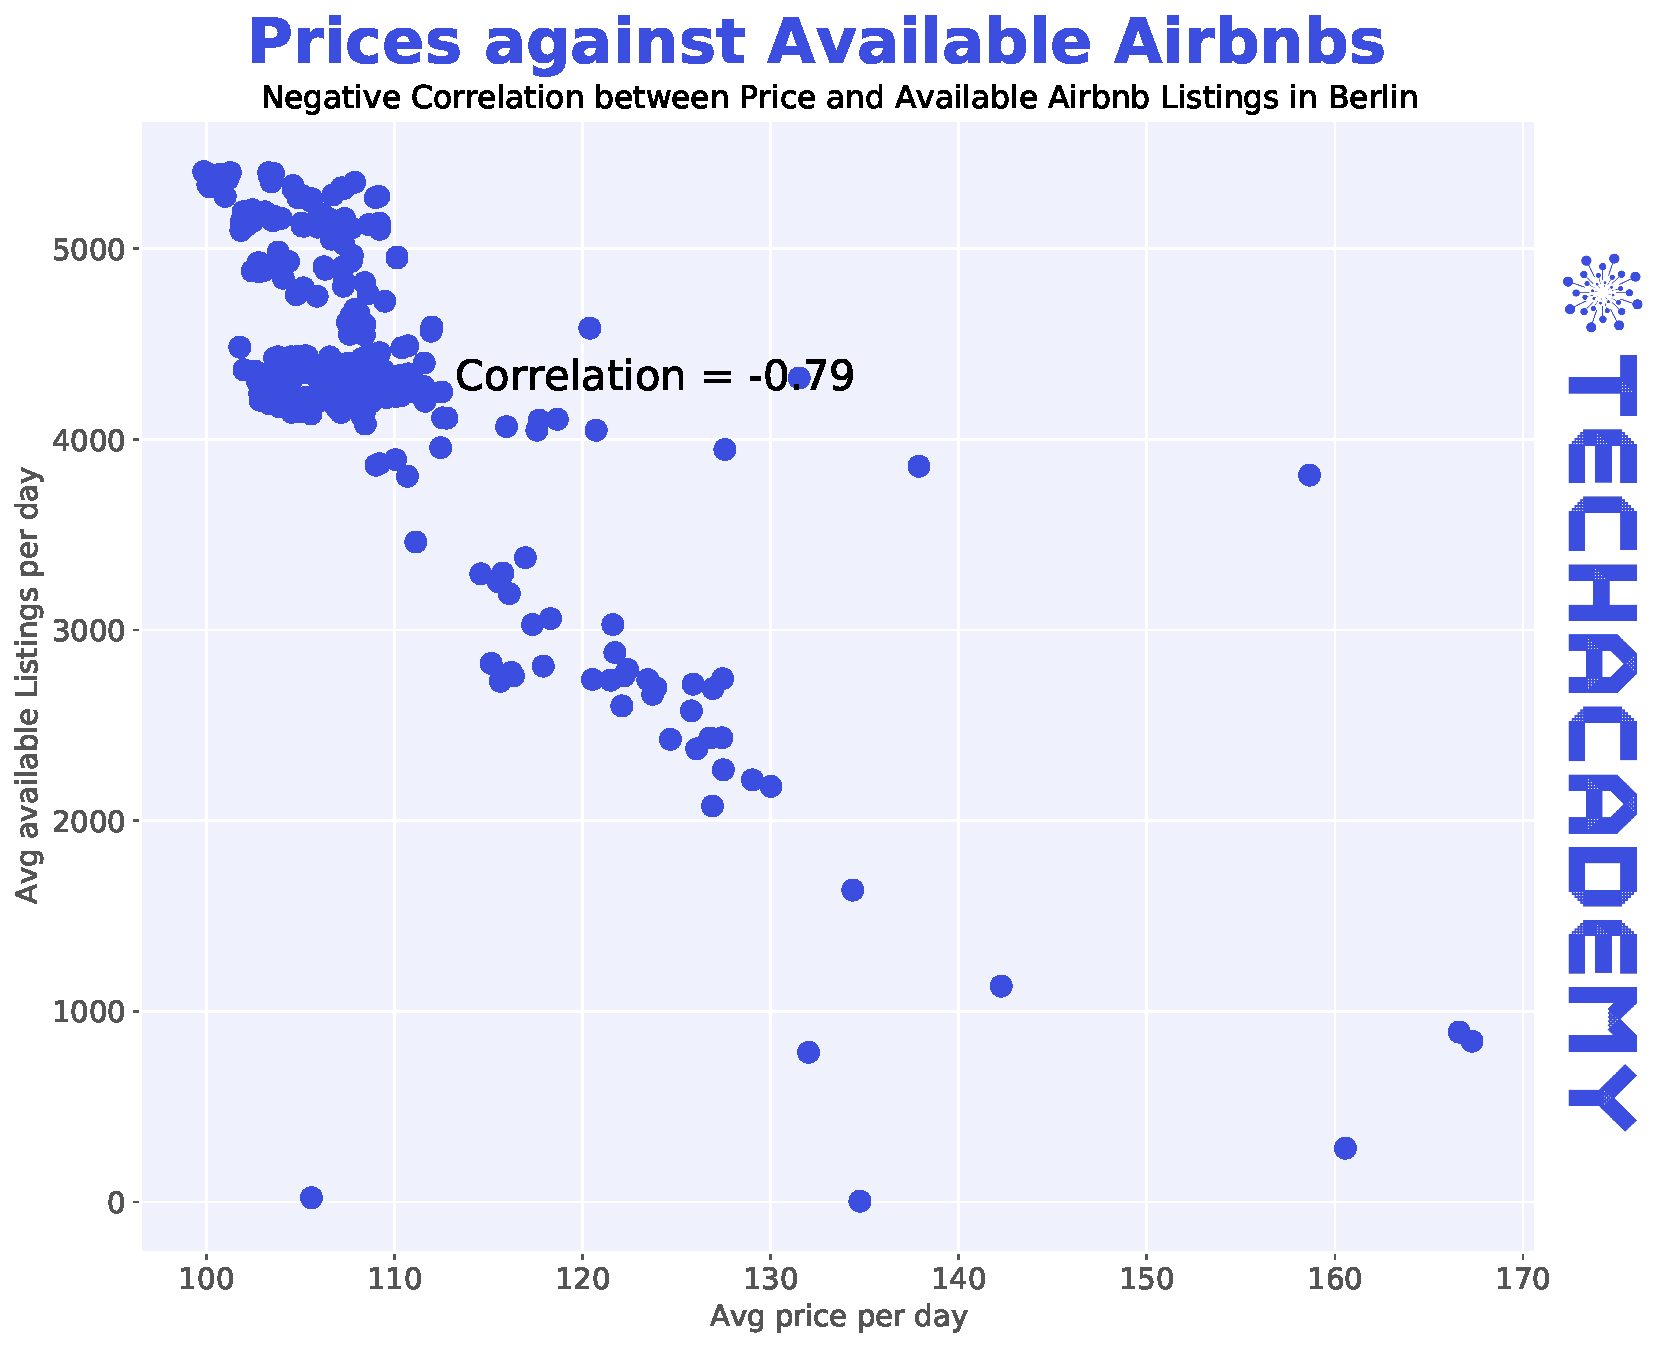
\includegraphics[width=1\linewidth]{plot/01_python/corr_availability_price} \end{center}

\textbf{Answer:} ``The correlation coefficient shows \ldots{}''.

\begin{tips}r
Have a look at \texttt{ggplot2} and plot a scatter plot with \texttt{geom\_point()}.
Use the stats function \texttt{cor(x,y),} for example, to calculate the correlation coefficient between two variables.

\end{tips}

\begin{tipsp}p
You can use matplotlib's scatter plot for plotting and pandas's \texttt{.corr()} method to compute the correlation coefficient between two variables.

\end{tipsp}

\hypertarget{visualize-individual-airbnb-offers-with-the-listings-data-set}{%
\subsection{Visualize individual Airbnb Offers with the Listings Data Set}\label{visualize-individual-airbnb-offers-with-the-listings-data-set}}

Can we use the mean price of a neighborhood to measure popularity?
Perhaps\ldots{} In the next section, you will compute the average price for each neighborhood, and since, as an (aspiring) Data Scientist, you love numbers and stats, you also want to compute the price variances for these neighborhoods.

Start by importing the \texttt{listings} dataset.
First, you will need to clean the \texttt{price} column.
After that, we can take a closer look at the price structure of the various neighborhoods.

Second, we would like to know the average price and corresponding standard deviation for each neighborhood.
Please list the names of the different parts of the city and their \texttt{mean} and the \texttt{sd} for that purpose.

\begin{tips}r
For this task, you can reuse \texttt{dplyr}-functions like \texttt{group\_by()} or \texttt{summarize()}.

\end{tips}

\begin{tipsp}p
Once again, you can use the .\texttt{groupby()} method to group by neighborhood and apply an aggregation function for calculating the standard deviation.
A very similar function exists for calculating the mean values.
Filter both data frames by the price column.

\end{tipsp}

Next, we now want to visually compare the price distribution for the, on average, most expensive district with the least expensive district.
For this task, think about the different types of plots that you have explored in your courses and find the most suited plot type for this type of visualization.
Once you have created your custom visualization, you will probably have to filter out some observations with extremely high prices (outliers) to get a more meaningful plot.

Your plot could end up looking like this:

\begin{center}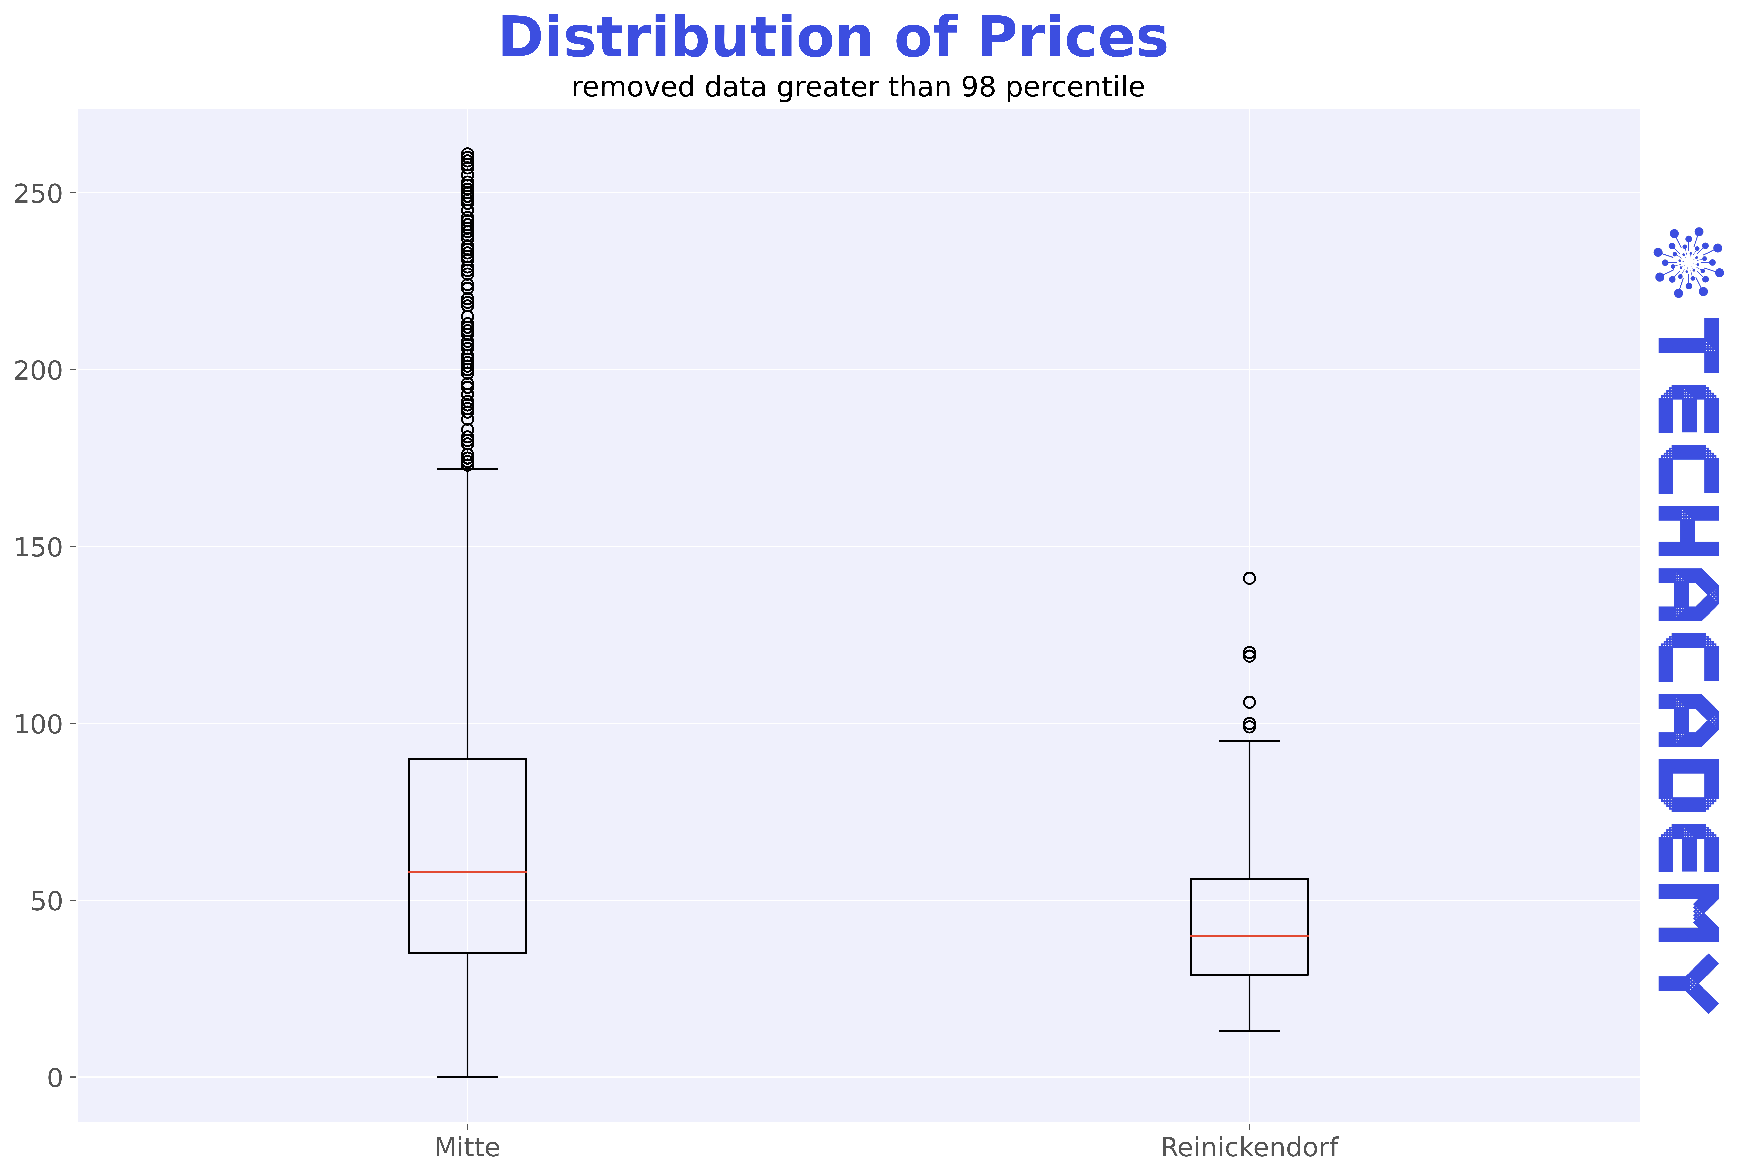
\includegraphics[width=1\linewidth]{plot/01_python/box_plots} \end{center}

\begin{tips}r
In \texttt{ggplot2} graphics, you can easily filter in the plot specifications with \texttt{xlim()} or \texttt{ylim()}.

You could use \href{https://www.r-graph-gallery.com}{this resource} to remind yourself of the different visualizations available in \texttt{R}.

\end{tips}

\begin{tipsp}p
One way to find the, on average, most expensive neighborhood is to sort the mean price column in descending order.

For plotting: The Matplotlib documentation is an excellent source of inspiration with many examples, including code that generated them.

\textbf{Note:} If you do not want to remove outliers, the plot could end up looking very strange.
In that case, it is best to create two different plots, i.e., one for each neighborhood.

\end{tipsp}

But wait!
Until now, we focused much on prices.
What about customer preferences?
Next, we will use the average number of reviews to indicate the ``hotness'' 🔥 of an area in your city!

\hypertarget{analyzing-number-of-reviews-per-neighborhood}{%
\subsection{Analyzing Number of Reviews per Neighborhood}\label{analyzing-number-of-reviews-per-neighborhood}}

In the previous part, you got to know and visualize the \texttt{listings} data set.
However, a critical piece of information is missing from this data that we could use to measure popularity.
How about using the number of reviews?

We first start by computing the average number of reviews per apartment.
Afterward, we will do the same for each neighborhood.
Calculating the number of reviews for each apartment could lead to a vital feature for price prediction.

Fortunately, we have another data set for each city, \texttt{reviews}, that recorded the apartment ID and the \texttt{date} for each review.
Our goal now is to count the number of reviews for each apartment and to keep them.
Since we can also find the \texttt{ID} in the \texttt{listings} data set, we can use that variable to merge the two data sets.

First, load your city's \texttt{reviews} data set into your workspace and take a closer look at it with the familiar functions.
Afterward, count the number of reviews per apartment.

\begin{tips}r
This works with the \texttt{table()} function or with \texttt{group\_by()} and \texttt{summarize()}.
Note, however, that you still have to convert the result of the \texttt{table()} function into a \texttt{data.frame} format for further processing.

\end{tips}

\begin{tipsp}p
Count the number of reviews per apartament (i.e.~per ``listing\_id'') with the functions you're already familiar with at this point.
You can use the groupby argument \texttt{as\_index=False} to avoid setting the column with listing ids as index, which might make live more easy when we merge data frames in later steps.

\end{tipsp}

To merge \texttt{reviews} with the \texttt{listings} data set, you have to rename the newly generated variables in the new data set.
Name the apartment \texttt{ID} analogous to the \texttt{listings} data set \texttt{id} and the number of reviews \texttt{n\_reviews}.

\begin{tips}r
You can do this task with the \texttt{rename()} function from the \texttt{dplyr} package.

\end{tips}

\begin{tipsp}p
Assign the new column names as a list to the \texttt{.column} attribute.

\end{tipsp}

If your data set looks similar to this, you can merge it with \texttt{listings}:

\begin{center}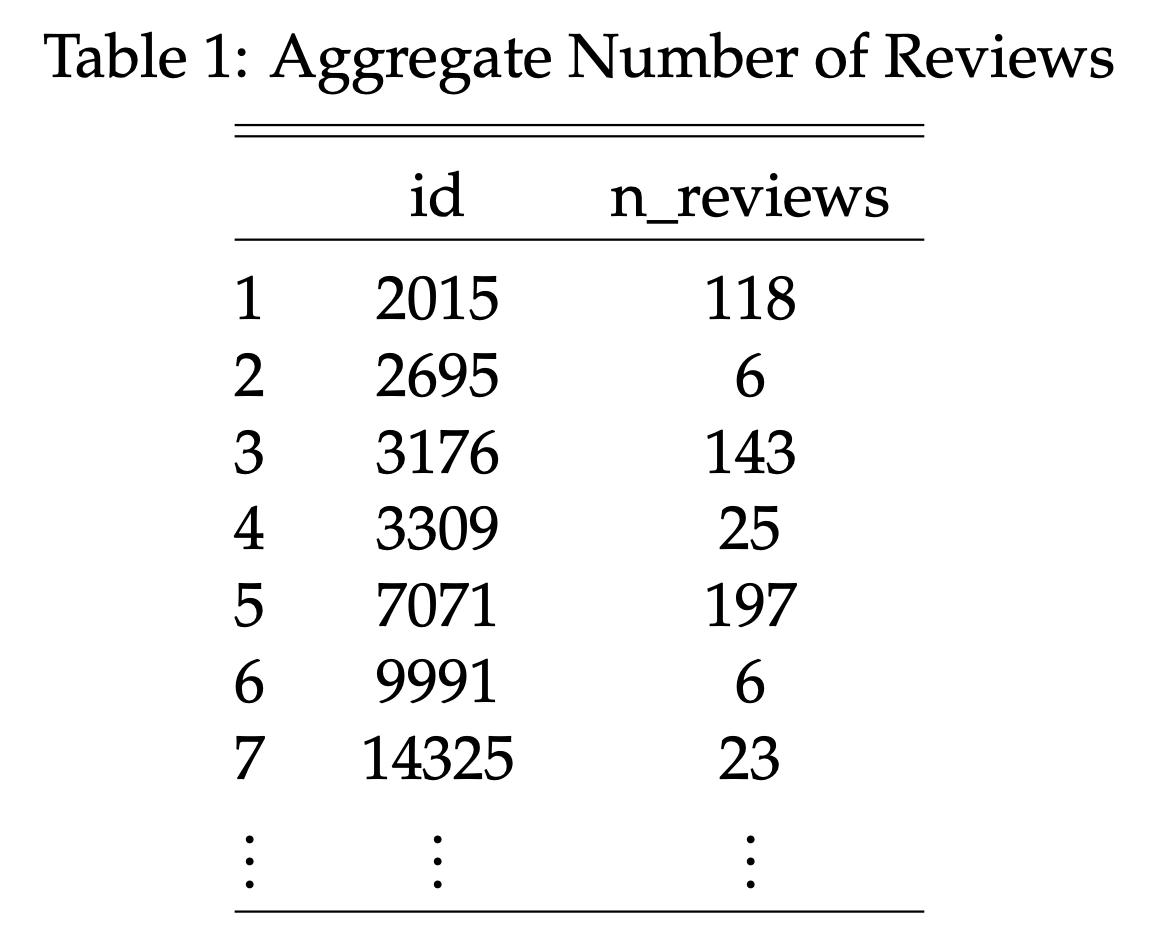
\includegraphics[width=0.4\linewidth]{plot/2_merging_table} \end{center}

\begin{tips}r
You can use the following function for merging:

\texttt{listings\_reviews\ \textless{}-\ merge(dataset1,\ dataset2,\ by\ =\ ...)}

\end{tips}

\begin{tipsp}p
Merge with \texttt{listings\_reviews=pd.merge(dataframe1,dataframe2,left\_on=...}.

\end{tipsp}

Now, look at the new data set.
Does each ID have exactly one entry with the number of ratings?
Reduce the data frame to the columns listing id, neighborhood, and the number of reviews to better understand your data.

\hypertarget{your-first-barplot}{%
\subsubsection{Your First Barplot}\label{your-first-barplot}}

We now want to take a closer look at a minor part of the data set: What do the most reviewed apartments have in common?
Is it the location?

Extract the 200 most reviewed apartments.
One approach is to sort the data set in descending order according to \texttt{n\_reviews} first and then extract the first 200 entries into a new data set.

Now you can easily visualize the districts with the 200 most frequently reviewed apartments.
A bar plot is ideal for this.
Feel free to try other types of visualizations best suited to answer this question.

This is what the visualization could look like:

\begin{center}\includegraphics[width=1\linewidth]{plot/01_python/hbars_reviews} \end{center}

\begin{tips}r
The key commands that you can use for this within \texttt{ggplot()} are \texttt{geom\_bar()} and \texttt{coord\_flip()}.

\end{tips}

\begin{tipsp}p
You can plot bar plots with both pandas and matplotlib.
If you chose to plot with matplotlib, you could use the \texttt{plt.barh()} method.
Additionally you might want to use methods like \texttt{.set\_yticks()}, \texttt{.set\_yticklabels()} and \texttt{.invert\_yaxis()}.

If Python throws you an \texttt{AttributeError}, then try working with the \texttt{plt.gca()} method.

\end{tipsp}

\hypertarget{visualization-with-maps}{%
\subsection{Visualization with Maps}\label{visualization-with-maps}}

This part will be the final and most advanced part of the EDA and the most rewarding.
Anyone who knows the Airbnb website has probably also seen their map showing the location of all apartments.
We can do the same!
The only difference is that our data gives us the option to show what interests us 😉

To reduce complexity, use the data set filtered in the \href{https://tech-academy-ev.github.io/exploratory-data-analysis.html\#your-first-barplot}{task before} with the 200 most frequently reviewed apartments.

If you have not solved that previous task yet, select 200 listings according to other criteria or at random to complete this task.

Your map could look like this:

\begin{center}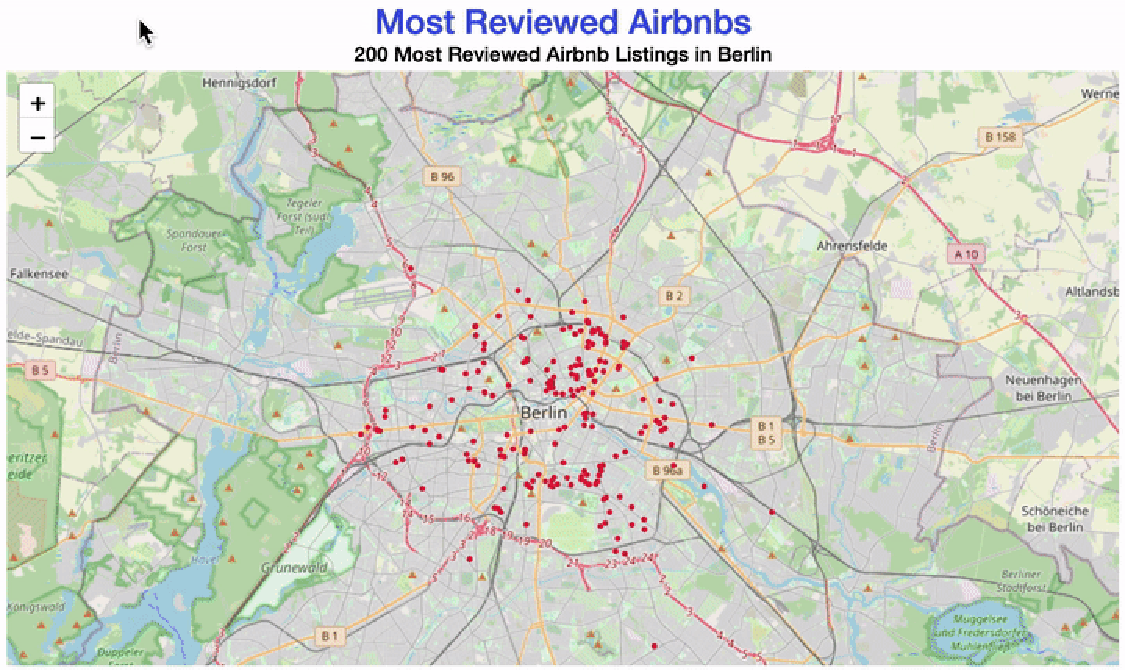
\includegraphics[width=1\linewidth]{plot/01_python/map_circles} \end{center}

\begin{tips}r
There are different ways of creating a map with \texttt{R}.
Although we plotted our example using the \texttt{leaflet} package, the following tips will be about the \texttt{ggmap} package as it is easier to use.

Before you can download map material via an API interface, you have to define the corners of the map as coordinates.

First, define the height and width of the included coordinates.
In the next step, you can specify the exact corners relative to the coordinates in the data set.

\begin{verbatim}
height <- max(...) - min(...)
width <- max(...) - min(...)
\end{verbatim}

You can then define a vector, which you can call \texttt{berlin\_borders}, as we did for Berlin's example.
We can use such a vector to determine the values for the edges of the map.
You can add a small safety margin to the respective minimum or maximum of the coordinates.
Play around with the factors later to find a good section of the map.

\begin{verbatim}
berlin_borders <- c(bottom = min(listing_top200$latitude) - 0.1 * height,
top = max(listing_top200$latitude) + 0.1 * height,
left = min(listing_top200$longitude) - 0.1 * width,
right = max(listing_top200$longitude) + 0.1 * width)
\end{verbatim}

Then, we can download the defined map section from the service provider Stamen Maps with the \texttt{get\_stamenmap()} function and save it in an \texttt{R}-object.
Now you just need to plot it!

\end{tips}

\begin{tipsp}p

We are going to use yet another library, this one is called Folium.
For this task you need to work with its documentation which you can find online.

Use folium's \texttt{Circle} to draw a circle for each apartment at its location coordinates.
You will need to implement a \texttt{for}-loop to iterate over all 200 apartments.

\begin{verbatim}
# Initiate the map
m = folium.Map(
    location=[52.5, 13.4],  # Berlin Coordinates
    zoom_start=11,
    tiles='Stamen Toner'  # Map Style
)

# Use a for-loop to plot circles
for idx, row in df.iterrows() :
    # Your code here

m  # Displays the map
\end{verbatim}


\end{tipsp}

In addition to the coordinates, there is a lot of information about each listing in our data.
This time, implement a pop-up window to display more details about each Airbnb apartment.

Your map should now look similar to this one:

\begin{center}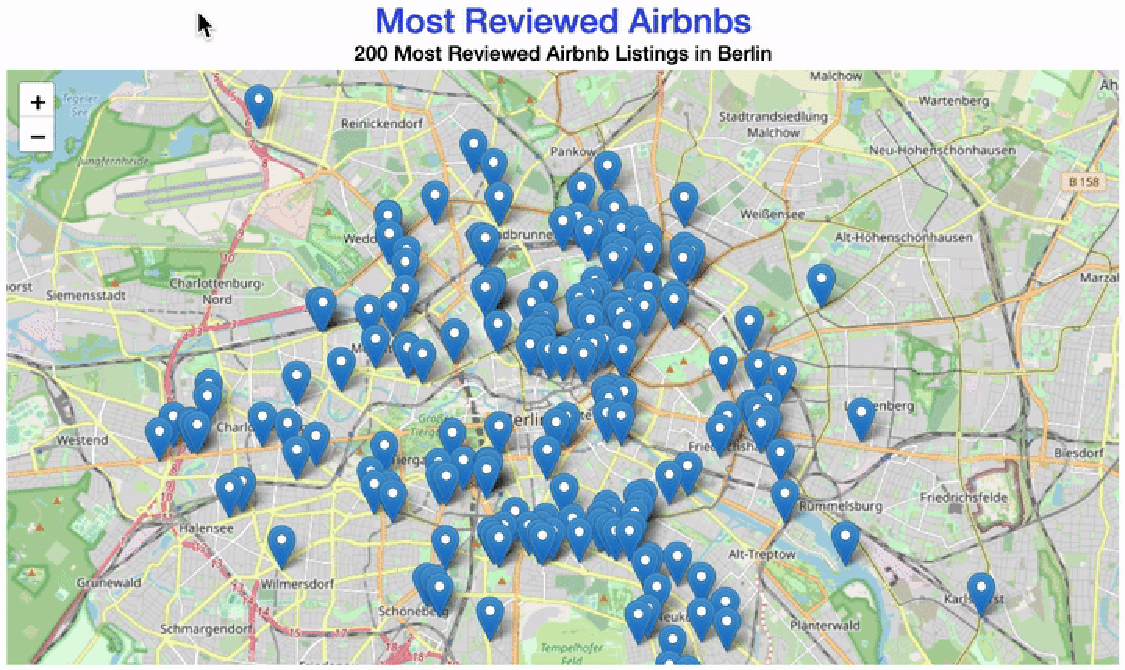
\includegraphics[width=1\linewidth]{plot/01_python/map_popup} \end{center}

\begin{tips}r
This time, we created the plot with \texttt{leaflet}.
Why don't you try to find information on the package online?

You can create a basic map with leaflet and add additional layers by following these simple steps:

\begin{verbatim}
m <- leaflet() %>%
  addTiles() %>% 
  addMarkers(lng= , 
             lat= , 
             popup= )
           
\end{verbatim}

Do \texttt{lng} and \texttt{lat} look familiar to you from a previous plot?

The \texttt{popup} is where the magic happens!
Can you make the map show you listings ID, type, price, review score, and number of reviews per apartment?

\end{tips}

\begin{tipsp}p

Once again, you will need to loop through each apartment.

This time however, the body looks more like this:

\begin{verbatim}
folium.Marker(
    [longitude, latitude], 
    popup="<i>some text here</i>", 
    tooltip='click me!'
).add_to(m)
\end{verbatim}


\end{tipsp}

For some analyzes, it is easier if you don't just see points but their distributions on a map.
For example, to see many apartments in a small space, you can display the apartment density.
Why not plot a heatmap?

\begin{tips}r
You are now familiar with two packages that can plot maps in \texttt{R}.
If you want to use \texttt{ggmap} to create such a two-dimensional density plot, you can use the \texttt{geom\_density2d()} and \texttt{stat\_density2d()} packages on the map.

If you don't know precisely how to fill the individual arguments, you can always Google for more help.

\end{tips}

\begin{tipsp}p
No hints or tips here - it's up to you to study the documentation for \texttt{folium}'s heatmap and to come up with a (possibly) nice heatmap 😉

\end{tipsp}

\hypertarget{surprise-us-with-at-least-one-more-plot}{%
\subsection{Surprise Us! (With At Least One More Plot)}\label{surprise-us-with-at-least-one-more-plot}}

Be creative!

With the available data, you could do a ton of more stuff.
You could try to find the perfect listing that suits your needs and plot an availability calendar for that listing, perfect for your holiday planning!
You could further go into a more detailed price analysis or come up with other plots (e.g., distribution of room types per neighborhood, or even number of hosts who join Airbnb per month!).
Also, compare the results with your teammates!
How do things look like in other cities, compared to yours?

\textbf{Congratulations} -- based on your work with fundamental data transformations and many visualizations, you now have a solid understanding of the Airbnb offers in your city!
With this step, you have now completed the first part of the project!
If you are in the beginner group, you have now met your minimum requirements.
Nevertheless, we strongly recommend that you also have a look at the following part.
There you'll be developing methods to predict the price of an apartment!
Sounds exciting?

\newpage

\hypertarget{price-prediction-application-of-statistical-methods}{%
\section{Price Prediction -- Application of Statistical Methods}\label{price-prediction-application-of-statistical-methods}}

In the previous part you got a feel for the data set. You now know which variables are included and a few characteristic properties of the data set. But so far, we have only visualized the data set. In this section we go a step further and use statistical methods to predict the price of individual Airbnb apartments as accurately as possible.

In order to be able to compare your models at the end, we use a uniform metric according to which we can check the price predictions for accuracy. In our case this is the Root Mean Square Error (\(RMSE\)), i.e.~the root of the average squared difference between the predicted (\(\hat{y}_i\)) and actual value (\(y_i\)):

\[ RMSE = \sqrt{\frac{1}{N}\sum_{i=1}^{N}{(\hat{y}_i-y_i)^2}} \]

The closer the \(RMSE\) is to 0, the better your model predicts prices. In the following, your goal is therefore to reduce the \(RMSE\) of your various models as much as possible through continuous improvements.

We use the Airbnb listings data set, which contains features about apartments including prices. When we train our model with the data, we need to estimate how well our model predicts prices for listings it has never seen before. Therefore we split our data set into two parts - a train and a test set.

Here is a brief description of what you need each of the data sets for:

\begin{itemize}
\item
  \emph{train data} (70 \%): You use this training data set to train your model. The model can learn the relationships between the variables based on the training data set that contains both, the variables needed to predict the prices and also the actual prices themselves.
\item
  \emph{test data} (30 \%): With this test data set you can test how well your model predicts the price using data that has not been seen before. This will help you for example with recognizing under- or overfitting.
\end{itemize}

\begin{tips}r
There are multiple ways to split/partition the data set in R. You could, e.g., use \texttt{createDataPartition()} function from \{caret\}, \texttt{sample.split()} function from \{caTools\} or --- perhaps most intuitively --- \texttt{split\_train\_test()} function from \{healthcareai\}.

Make sure, however, to include the \texttt{set.seed()} function in your R code before randomly dividing the data set into train/test parts. \texttt{set.seed()} function allows you to reproduce randomness each time you re-run your code. That means that you always get the same (random) result -- a vital aspect of reproducibility within the scientific method.

\end{tips}

\begin{tipsp}p
The sklearn library has a function that you can use to split the data set, correspondingly

\begin{verbatim}
from sklearn.model_selection import train_test_split
X_train, X_test, y_train, y_test = train_test_split(...)
\end{verbatim}

Make sure to set the random seed parameter, such that the train and test data sets have the same values each time the method is called.

\end{tipsp}

\hypertarget{examine-correlation-between-the-variables-train}{%
\subsection{Examine Correlation Between the Variables (train)}\label{examine-correlation-between-the-variables-train}}

How are the individual variables related to each other? In other words, to what extent do the variables in the data set correlate with one another? Finding this out is extremely important for deciding which model specification to use later. A good place to start is to create a correlation matrix:

\begin{center}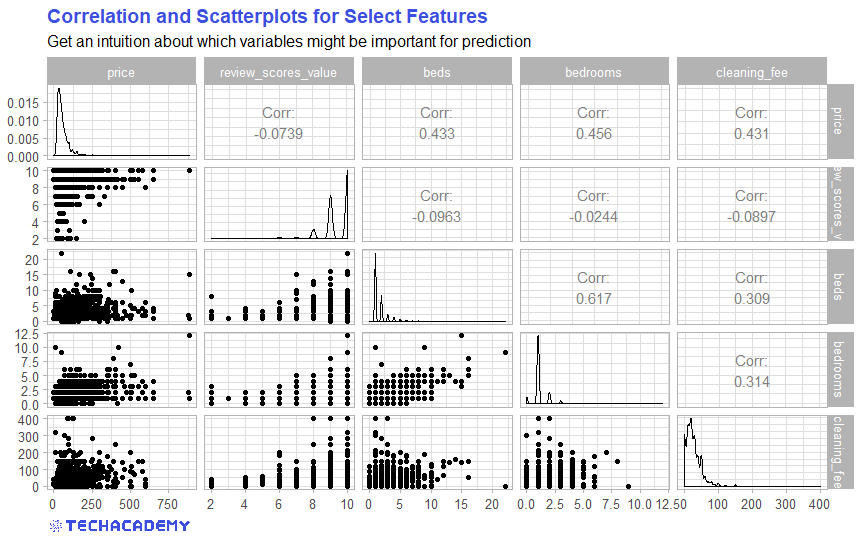
\includegraphics[width=1\linewidth]{plot/5_1_ggpairs} \end{center}

\begin{tips}r
Use the \texttt{cor()} function from the \{base\} R to create a correlation matrix. Select all numerical variables in your data set with the help of \texttt{sapply()} or \{dplyr\}'s \texttt{select()} and create a correlation matrix.

Alternatively, use the \texttt{ggcorrplot()} from the same-name \href{https://cran.r-project.org/package=ggcorrplot}{\{ggcorrplot\}} package.

Check out \href{http://jamesmarquezportfolio.com/correlation_matrices_in_r.html}{this article} by James Marquez if you're curious about other ways to create a correlation plot in R.

\end{tips}

\begin{tipsp}p
A handy library for plotting correlation matrices is the seaborn library: \texttt{import\ seaborn\ as\ sns}.

Use its pairplot method and pass on the dataframe with the selected columns to visualize distributions and correlations.

Additionally, you may want to plot a heatmap with \texttt{sns.heatmap()} which makes it even easier to see correlations.

\end{tipsp}

Which of your examined variables correlates most with price and which seems to be more independent from price? You now have a first impression over which variables could be important for your model. So let's get to your first price prediction model!

\hypertarget{first-predictions-with-simple-regression-models-train}{%
\subsection{First Predictions with Simple Regression Models (train)}\label{first-predictions-with-simple-regression-models-train}}

Now you can make use of your statistical knowledge. You will need a method with which you can predict the price of an Airbnb apartment. A very simple first approach would be to use the average demand as the first prediction. However, this is almost certainly not the best prediction. In this case, your predicted price would be the same over all days and would ignore all factors that influence the price.

Ever heard of linear regression? That would be a much better approach. Now you can use your statistics skills. First set up a model with the dependent variable \texttt{price}. In the previous exercise you examined different variables. Now choose the variable with the highest correlation to price and use that as the only independent variable.

For example, your first regression model could look like this:

\[price_i = \beta_0 + \beta_1 bedrooms_i + \epsilon_i\]

\begin{tips}r
In \texttt{R} you can implement a simple linear regression with the function \texttt{lm()}. You then get the model summary with the \texttt{summary()} function.

\end{tips}

\begin{tipsp}p
Define both dependent (y\_train) and independent (X\_train) variables and clean the data if necessary.

For the next step the X\_train values need to be reshaped \texttt{.values.reshape(-1,1)}.
Note: If you use more then one feature you don't have to reshape your data.

Import \texttt{LinearRegression()} from \texttt{sklear.linear\_model} and train your model using \texttt{LinearRegression().fit()}.

\end{tipsp}

Does your independent variable have a statistically significant impact on apartment price? Probably yes, because we selected the variable most correlated with price. However, if we stick to this very simplified model, we are making a typical mistake: the so-called Omitted Variable Bias (OVB). To put it simply, we neglect (in statistics jargon: ``do not control for'') variables that have a significant influence on the dependent variable. One could suspect that other influencing factors also play a large role in price setting. If we do not include them, the estimate of the effect of \texttt{bedrooms}is biased and thus hardly useful. In our case this is not a big problem for the time being, since we are not interested in causal effects, but rather in the best possible prediction. Your statistics professor would almost certainly object to such a model. Nonetheless, with just a single explanatory variable, this model will not necessarily predict the price well.

One possible solution is to simply include the omitted variables in the model -- how practical that these are already included in the data set. So let's set up a somewhat more extensive model that includes one more variable:

\[price_i = \beta_0 + \beta_1 bedrooms_i + \beta_2 cleaning\_fee_i + \epsilon_i\]

Now compare the results of the two models. Does the larger model explain a higher proportion of the variance in price? In other words, which model shows the higher value for the \(R^2\) measure?

\begin{tips}r

You can easily include such LaTeX tables in your RMarkdown document with the \texttt{stargazer} package:

\begin{center}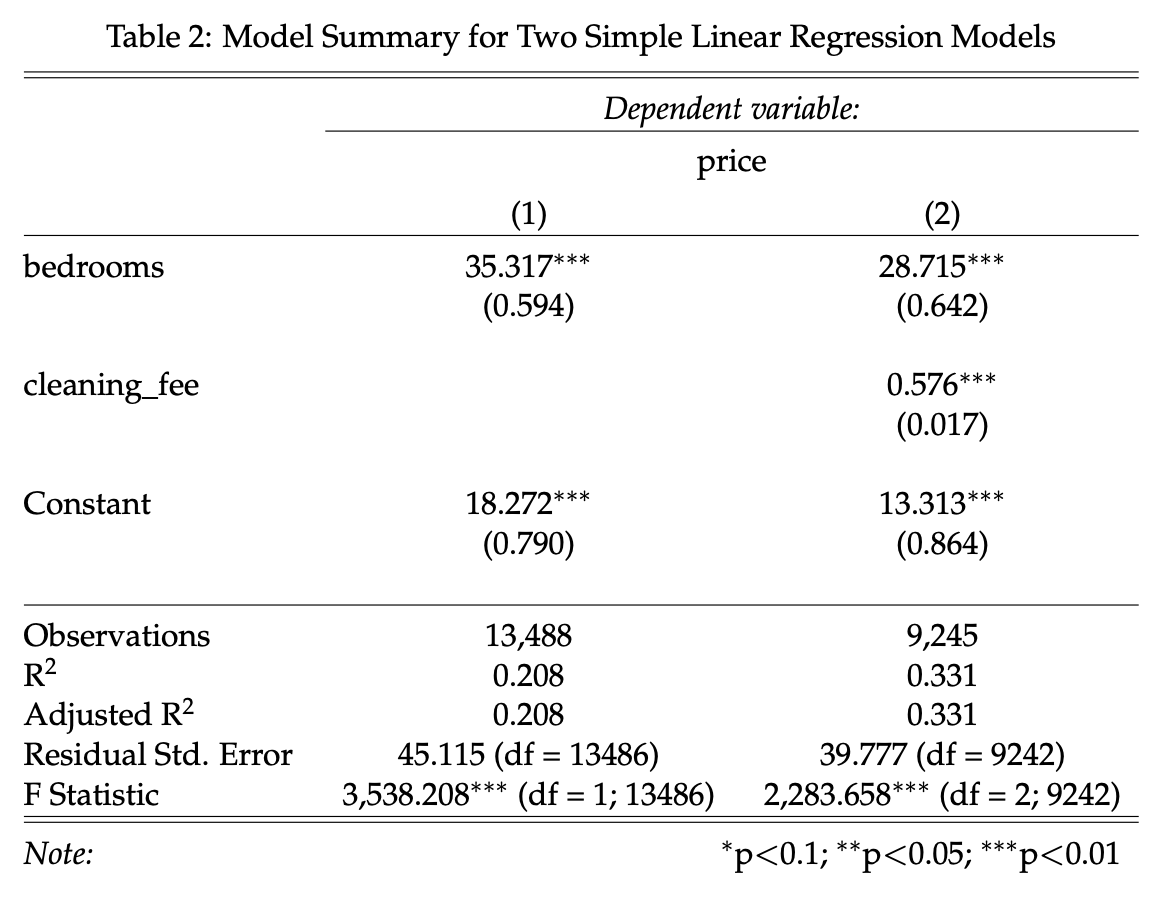
\includegraphics[width=1\linewidth]{plot/5_table} \end{center}


\end{tips}

\begin{tipsp}p
Apply the \texttt{.summary()} method on the fitted model estimator.

\end{tipsp}

\hypertarget{from-training-to-testing-making-predictions}{%
\subsection{From Training to Testing -- Making Predictions}\label{from-training-to-testing-making-predictions}}

You have now trained your first model with the training data set. But how well does the model handle data that it has not seen yet? This is a very important test to evaluate the quality of your model.

Has your model only ``memorized'' the existing patterns in the training data set?
Then the relationships from the training data set would not be transferable to the test data set. With so-called overfitting, the model was trained too closely to the training data set and therefore provides poor predictions for unknown data -- for example the data in your test and validation data sets.

On the other hand, there is also the problem of underfitting: Your model has not sufficiently learned the actual relationships between the data and therefore makes poor predictions in the test data set. So it is important to find a balance between the two problems.

Now the distinction between training and test data sets becomes important. As a reminder: we use train data to train a model and the test data to ultimately test the quality of our model.

Now load the data set \texttt{test} in addition to the data set \texttt{train} that you have already used. In order to test your model on previously unseen data, you can apply the model to the test data set.

\begin{tips}r

Use the \texttt{predict} function for this:

\texttt{predicted\_price\ \textless{}-\ predict(your\_saved\_model,\ your\_test\_data\_frame)}

You have now created a vector with all price predictions for the test data set. You can now compare this with the actual values for \texttt{price} from \texttt{test}.

In order to use a uniform comparison metric, please use the following function to measure your prediction accuracy:

\begin{verbatim}
# Function that returns Root Mean Squared Error while ignoring NAs
rmse <- function(actual, predicted) {
sqrt(mean((predicted - actual)^2, na.rm = TRUE))
}
\end{verbatim}


\end{tips}

\begin{tipsp}p

After training, import the data from the \texttt{test.csv} file, define both variables \texttt{X\_test}and \texttt{y\_test}, and create a vector with price predictions applying \texttt{.predict(X\_test)} on your model. Store your prediction in the variable \texttt{predicted\_price}.

Finally, compare your predicted values with the test values:

\begin{verbatim}
from sklearn.metrics import mean_squared_error
# Function that returns Root Mean Squared Error while ignoring NaNs
rmse = mean_squared_error(y_test, predicted_price, squared=False)
\end{verbatim}


\end{tipsp}

Now compare both regression models. Does the larger model have better prediction accuracy, i.e.~a lower \(RMSE\)? Now you have a benchmark for your more advanced models, which you can beat in the next part.

\hypertarget{apply-advanced-machine-learning-algorithms}{%
\subsection{Apply Advanced Machine Learning Algorithms}\label{apply-advanced-machine-learning-algorithms}}

Now that you have created and tested an initial prediction using a simple regression model, you can now apply more advanced methods. The goal is still to get the lowest possible \(RMSE\) when applying the model to the test data set. Now look at at least one other algorithm and then see if that gives you a more accurate prediction (expressed as a lower \(RMSE\)). You can find inspiration for this in the advanced DataCamp courses, which are listed at the beginning of the project guide. There are no limits for you -- you can refine the regression using certain methods (e.g.~LASSO) or set up a random forest model or a neural network. It is usually a good idea to briefly recall the functionality of the respective algorithms and to consider whether this methodology makes sense in this case with a continuous prediction variable.

At this point, a disclaimer is appropriate: Our data set has a substantial part of missing observations (\texttt{NA}) for many variables. Some machine learning algorithms require a complete set of data with no missing values, while others can do well with a smaller number. If you get into trouble about the missing values, check whether you can impute the missing values. Which method is best for imputation depends heavily on your prediction algorithm.

You can also get a noticeable gain in predictive power by modifying existing variables or generating new variables from the data set (``feature engineering''). For example, we could imagine that the distance from an apartment to the city center has a significant impact on the price. However, this variable is not
included in our data set. You can write a simple function that uses the two coordinate variables to calculate the distance to the center of Berlin and appends this to the data set as a new variable.

Always compare the \(RMSE\) of your advanced models with each other, as well as with the benchmark regression model from before.

Congratulations! You've made it to the end of your TechAcademy Data Science project. After visualizing the data in the first part, you've also set up predictive models in this section. If you stuck around until this part and managed to code the better part of the exercises, you've definitely earned your certificate! We hope you had fun learning Data Science with this data set and you enjoyed it -- at least the parts where you didn't get stuck forever because of some unexplainable coding error. Don't forget to send your project results and the prediction-csv file you just generated to our project submission email address before the deadline.

\newpage

\hypertarget{exercise-checklist}{%
\section{Exercise Checklist}\label{exercise-checklist}}

This checklist should help you keep track of your exercises. Remember that you have to hand in satisfactory solutions to at least two-thirds of the exercises. If you're part of the beginner track, this refers to two-thirds of part A (EDA) only. If you're part of the advanced track, you have to hand in at least two-thirds of both individual parts A and B. Hence, you cannot hand in 100 percent of the first part and only 50 percent of the second one. You'll need more than 66\% in each one for a certificate. After all, you're not that advanced if you only did half of it, right?

\textbf{Part 1: Exploratory Data Analysis (Beginner + Advanced Tracks)}

\begin{enumerate}
\def\labelenumi{\arabic{enumi}.}
\item
  Load the \texttt{calendar} data set and get an overview of it
\item
  Fix the variables: \texttt{price}, \texttt{available}, and \texttt{date}
\item
  Transform and aggregate the \texttt{calendar} data set to, e.g., \texttt{avail\_by\_date}
\item
  Show the number of available Airbnb apartments in a simple line plot
\item
  Create a calendar plot to visualize the availability of Airbnb listings
\item
  Calculate the correlation coefficient (\emph{r}) between \texttt{available} and \texttt{price} and plot both variables
\item
  Import \texttt{listings} data set, clean \texttt{price} column, and list the names of the different parts of the city and their \texttt{mean} and the \texttt{sd}
\item
  Visually compare the price distribution for the, on average, most expensive district with the least expensive district
\item
  Import \texttt{reviews} data set, count the number of reviews per apartment, and store it in a new variable, e.g., \texttt{n\_reviews}
\item
  Merge \texttt{reviews} with the \texttt{listings} data set and reduce the number of columns in a resulting data set
\item
  Extract and plot the 200 most reviewed apartments, e.g., using a barplot
\item
  Map the 200 most frequently reviewed (or random) Airbnb apartments
\item
  Implement a pop-up window to display more details about each Airbnb apartment on your map
\item
  Use a heatmap to visualize many apartments in a small space
\item
  Surprise us with your plot of choice!
\end{enumerate}

\textbf{Part 2: Price Prediction Using Statistical Methods (motivated Beginner + Advanced Tracks)}

todo

\begin{enumerate}
\def\labelenumi{\arabic{enumi}.}
\item
  Visualize feature correlations in a correlation matrix/heatmap
\item
  Regression

  \begin{enumerate}
  \def\labelenumii{\alph{enumii}.}
  \item
    Simple regression model using one variable
  \item
    Improve your model using more features
  \end{enumerate}
\item
  Test your model

  \begin{enumerate}
  \def\labelenumii{\alph{enumii}.}
  \item
    Use test data set to predict prices of the apartments
  \item
    Compare your predictions with the actual values
  \item
    Train a new model using a more advanced method, send us your model and the predictions of your best model
  \end{enumerate}
\end{enumerate}

\newpage

\hypertarget{whats-next-in-your-data-science-career}{%
\section{What's Next in Your Data Science Career?}\label{whats-next-in-your-data-science-career}}

At the end of your TechAcademy semester, you've successfully coded your way through a whole Data Science project. You liked what you did and would like bring your skills to the next level? Then this section provides you with many useful resources to deepen your knowledge in Data Science in general or Python and R in particular. The first section is useful for every aspiring Data Scientist, while the two following boxes introduce you to some language-specific resources. If you've come across some other useful materials that we didn't mention here, feel free to contact us -- this list is far from complete!

\hypertarget{data-science-in-general}{%
\subsection{Data Science in General}\label{data-science-in-general}}

\hypertarget{version-control-with-git}{%
\subsubsection*{\texorpdfstring{Version Control with \href{https://github.com/}{Git}}{Version Control with Git}}\label{version-control-with-git}}
\addcontentsline{toc}{subsubsection}{Version Control with \href{https://github.com/}{Git}}

If you're serious about data science, you will need Git. Better learn it early and start enjoying and appreciating it before it's too late and you're pressured into learning it on the fly! Every project you do should be accompanied by a VCS (Version Control System) like Git. Regardless if you're working alone or with a big group of developers. No matter whether you write ten lines of code or a really complex program. With Git, you can keep track of all your changes. It's like a Dropbox/Google Drive for developers, but way better. Pro-Tip: Get free GitHub Pro as a Student with the \href{https://education.github.com/pack}{GitHub Student Developer Pack}. Besides all the perks of GitHub Pro, you'll also free access to many other great tools. See the respective tutorials on how to set up your Git workflow.

\hypertarget{advice-for-non-traditional-data-scientists}{%
\subsubsection*{\texorpdfstring{Advice for \href{https://blog.shotwell.ca/posts/learning_data_science/}{Non-Traditional Data Scientists}}{Advice for Non-Traditional Data Scientists}}\label{advice-for-non-traditional-data-scientists}}
\addcontentsline{toc}{subsubsection}{Advice for \href{https://blog.shotwell.ca/posts/learning_data_science/}{Non-Traditional Data Scientists}}

Important advice from Gordon Shotwell, a former lawyer, on what it takes to have a successful data science career coming from a non-computer science background. Extremely encouraging and helpful read on what you should and shouldn't do to reach that goal.

\hypertarget{learn-from-great-data-scientists-on-kaggle}{%
\subsubsection*{\texorpdfstring{Learn from Great Data Scientists on \href{https://www.kaggle.com/}{Kaggle}}{Learn from Great Data Scientists on Kaggle}}\label{learn-from-great-data-scientists-on-kaggle}}
\addcontentsline{toc}{subsubsection}{Learn from Great Data Scientists on \href{https://www.kaggle.com/}{Kaggle}}

Kaggle is a platform that hosts data science challenges. The great thing about it is that you can browse through many clever solutions to tricky machine learning tasks. And of course, you can also join the competition and measure your predictions with others. There are plenty of both Python and R notebooks.

\hypertarget{r}{%
\subsection{R}\label{r}}

\begin{tips}r
\textbf{Install R and RStudio Locally}

RStudio.Cloud is great for getting started with R without having to worry about installing anything locally. Sooner or later you will have to install everything on your own computer. Here's a \href{https://www.datacamp.com/community/tutorials/installing-R-windows-mac-ubuntu}{DataCamp tutorial} on how to do that.

\textbf{Version Control with Git}

RStudio has a nice interface that lets you enjoy the perks of Git without ever having to touch the command line -- sounds great, does it? Learn how to set up the Git \& R workflow with \href{https://happygitwithr.com/}{Happy Git with R}.

\textbf{\href{https://www.r-graph-gallery.com/}{R Graph Gallery}}

Get inspiration to take your plotting to the next level. Includes code to reproduce the plots.

\textbf{Follow the R Master Himself and the R Community}

Hadley Wickham was and continues to be extremely influential on the development of R and its rise to one of the most popular data science languages. He's behind many tools that we taught you in this semester, especially the tidyverse (including great packages such as ggplot2 and dplyr). Follow him \href{https://twitter.com/hadleywickham}{on Twitter} to get great R advice and keep up to speed with everything new to R. Following the many people behind R (not only Hadley) is a great way for acquiring deeper understanding of the language and its developments.

\textbf{Join the \href{https://www.meetup.com/r-frankfurt/}{Campus useR Group in Frankfurt}}

There's a quite active R community in Frankfurt that meets once a month. It's open for students, professors, industry practitioners, journalists, and all people that love to use R. In those meetings, you'll hear about other's work, discuss new developments, and ask questions.

\textbf{Listen to R Podcasts}
Another great way to easily keep up with new developments in the Data Science/R community. Check out
\href{http://nssdeviations.com/}{Not So Standard Deviations} or \href{https://r-podcast.org/}{the R-Podcast}

\end{tips}

\hypertarget{python}{%
\subsection{Python}\label{python}}

\begin{tipsp}p
\textbf{Install Python Locally}

Until now you've only programmed using JupyterHub on the TechAcademy Server. A next step would be to install Python and Jupyter locally on your computer. This \href{https://docs.anaconda.com/anaconda/install/}{link} contains the necessary information on how to install the software on Windows, iOS or Linux.

\textbf{Choosing the Right Editor}

Using Jupyter is especially useful for short data analyses. But sometimes you want to write longer scripts in Python. In these cases, it is often more convenient to use a code editor instead of Jupyter. \href{https://realpython.com/learning-paths/perfect-your-python-development-setup/}{This tutorial} highlights the positive aspects of such an editor and how to choose the right one for you. Pro-Tip: Also check out the other tutorials on \href{https://realpython.com/}{Real Python} and check out the Community Version of ``PyCharm'' which is the most common Python IDE (Integrated Development Environment.

\textbf{\href{https://python-graph-gallery.com/}{Python Graph Gallery}}

Get inspiration to take your plotting to the next level. Includes code to reproduce the plots.

\textbf{More Advanced Python Concepts}

You know the basic data structures in Python like lists and dictionaries. What are the next steps to improve your knowledge? \href{https://book.pythontips.com/en/latest/index.html}{This website} gives good explanations for slightly more advanced concepts which can be very useful from time to time.

\textbf{A Deeper Understanding}

If you want to get a deeper understanding of the Python programming language and into typical algorithms which are used in the field of Data Science, this \href{https://github.com/ab-anand/py-books/blob/master/Data\%20Science\%20from\%20Scratch-\%20First\%20Principles\%20with\%20Python.pdf}{free book} can be a good starting point.

\textbf{Writing Beautiful Python Code}

``My code doesn't look nice, but it works!''
This might work for yourself, but often you will work on code with other people. But even if you're just coding for yourself it's a good idea to follow the PEP8 style guide. It's a useful convention on how to structure and code in Python. You'll find useful resources for PEP8 \href{https://realpython.com/python-pep8/}{here} and \href{https://www.python.org/dev/peps/pep-0020/\#id2}{here}.

\textbf{Listen to Python Podcasts}

When you don't have time for books you can listen to \href{https://talkpython.fm/home}{Talk Python} or the \href{https://www.pythonpodcast.com}{Python Podcast}.

\end{tipsp}

  \bibliography{book.bib,packages.bib}

\end{document}
